% =====================================================================
%  Mecánica Clásica — Sesión 11, Tema 1
%  Cuerpo rígido: velocidad angular y ángulos de Euler
%  L. A. Núñez — Escuela de Física, UIS
%
%  Codificación: UTF-8.   Compilar con: pdflatex (dos pasadas).
%
%  VERSIONES
%    \instructorfalse  -> versión para estudiantes (sin soluciones)
%    \instructortrue   -> agrega el apéndice con soluciones, errores
%                         frecuentes, clave de la actividad IA y rúbrica
%
%  NOTACIÓN (unificada en todo el documento; ver la diapositiva
%  "Notación de esta clase")
%    S  = (x, y, z)        sistema del laboratorio (inercial), origen O
%    S~ = (x_1, x_2, x_3)  sistema fijo en el cuerpo, origen en el CM
%    \Rot                  matriz de Euler, componentes en S -> en S~
%    Omega_x, Omega_y, Omega_z   componentes de Omega en S
%    Omega_1, Omega_2, Omega_3   componentes de Omega en S~
%    d\bm{\Phi}            rotación infinitesimal (no confundir con phi)
%  Para volver a la notación anterior (U~) basta cambiar \Rot abajo.
% =====================================================================

\documentclass[spanish]{beamer}
\usepackage[utf8]{inputenc}           % fuente en UTF-8
\usepackage[spanish]{babel}
\usepackage{amsmath,amssymb,mathtools}
\usepackage{bm}                       % vectores griegos en negrita
\usepackage{graphicx}
\usepackage{textpos}
\usepackage{listings}                 % código en el apéndice del instructor

\usetheme{Madrid}
\usecolortheme{beaver}

% ---------------------------------------------------------------------
%  Versión: estudiante / instructor
% ---------------------------------------------------------------------
\newif\ifinstructor
\instructorfalse        % <-- cambiar a \instructortrue para la versión docente

% ---------------------------------------------------------------------
%  Logo institucional (si el archivo no existe, simplemente se omite)
% ---------------------------------------------------------------------
\newcommand{\logoUIS}{/Users/luisnunez/Dropbox/MisDocumentos/UIS/UISImagenInstitucional/UISLOGO.png}
\newcommand{\insertaLogo}{%
  \IfFileExists{\logoUIS}{\includegraphics[height=0.4in,keepaspectratio]{\logoUIS}}{}}
\addtobeamertemplate{frametitle}{}{%
  \begin{textblock*}{100mm}(.85\textwidth,-1cm)\insertaLogo\end{textblock*}}

% ---------------------------------------------------------------------
%  Macros de notación
% ---------------------------------------------------------------------
\providecommand{\sen}{\operatorname{sen}}       % seno en castellano
\newcommand{\vect}[1]{\mathbf{#1}}              % vector latino
\newcommand{\uv}[1]{\hat{\mathbf{#1}}}          % vector unitario
\newcommand{\bOmega}{\bm{\Omega}}               % velocidad angular
\newcommand{\dPhi}{d\bm{\Phi}}                  % rotación infinitesimal
\newcommand{\Rot}{\mathbb{A}}                   % matriz de rotación (S -> S~)
% Matriz identidad: \mathds{1} si dsfont está instalado; si no, 1 en negrita
\IfFileExists{dsfont.sty}%
  {\usepackage{dsfont}\newcommand{\Id}{\mathds{1}}}%
  {\newcommand{\Id}{\mathbf{1}}}
\newcommand{\Inercia}{\mathbb{I}}               % tensor de inercia (próxima clase)
\newcommand{\Slab}{S}                           % sistema laboratorio
\newcommand{\Scue}{\tilde{S}}                   % sistema del cuerpo
\newcommand{\colLab}[1]{\mathsf{#1}}            % columna de componentes en S
\newcommand{\colCue}[1]{\tilde{\mathsf{#1}}}    % columna de componentes en S~
\newcommand{\tr}{\mathsf{T}}                    % transpuesta

% Estilo para el código Python (apéndice del instructor)
\lstset{language=Python, basicstyle=\ttfamily\fontsize{5}{5.8}\selectfont, columns=fullflexible,
  keepspaces=true, commentstyle=\color{gray}, showstringspaces=false,
  literate={á}{{\'a}}1 {é}{{\'e}}1 {í}{{\'i}}1 {ó}{{\'o}}1 {ú}{{\'u}}1 {ñ}{{\~n}}1}

% =====================================================================
\title[Cuerpo rígido: ángulos de Euler]{\textbf{Cuerpo rígido: velocidad angular y ángulos de Euler}}
\author[L.A. Núñez]{\textbf{Luis A. Núñez}}
\institute[UIS]{\textit{Escuela de Física, Facultad de Ciencias,} \\
  \textit{Universidad Industrial de Santander, Santander, Colombia} \\[2pt]
  \insertaLogo}
\date{\today}
% =====================================================================

\begin{document}

\maketitle

\begin{frame}
  \frametitle{Agenda}
  \tableofcontents
\end{frame}

% =====================================================================
\section{Objetivos y punto de partida}
% =====================================================================

\begin{frame}
  \frametitle{Objetivos de la clase}
  Al terminar esta clase usted debe poder:
  \begin{enumerate}
    \item<1-> \textbf{Justificar} que un cuerpo rígido tiene seis grados de libertad
          y \textbf{derivar} $\vect{v}=\vect{v}_{\mathrm{cm}}+\bOmega\times\vect{r}$.
    \item<2-> \textbf{Construir} la matriz de Euler $\Rot(\phi,\theta,\psi)$ en la
          convención $z$–$x$–$z$ e \textbf{interpretar} sus filas y columnas
          como cosenos directores.
    \item<3-> \textbf{Derivar} las componentes de $\bOmega$ en el sistema del
          cuerpo y en el laboratorio, y \textbf{verificarlas} por dos caminos
          independientes.
    \item<4-> \textbf{Analizar} el dominio de validez de los ángulos de Euler
          (singularidad en $\theta=0,\pi$).
    \item<5-> \textbf{Evaluar} críticamente una respuesta de un asistente IA sobre
          rotaciones, usando verificaciones físicas y matemáticas.
  \end{enumerate}
\end{frame}

\begin{frame}
  \frametitle{¿Qué necesitamos de clases anteriores?}
  \begin{itemize}
    \item<1-> \textbf{Ligaduras holónomas y grados de libertad:} un cuerpo rígido
          es un sistema de partículas con ligaduras $|\vect{r}_a-\vect{r}_b| = c_{ab}$.
          Los ángulos de Euler serán sus \textbf{coordenadas generalizadas} de orientación.
    \item<2-> \textbf{Sistemas en rotación:} para un vector $\vect{b}$ cualquiera,
          \[
            \left.\frac{d\vect{b}}{dt}\right|_{\Slab}
            = \left.\frac{d\vect{b}}{dt}\right|_{\Scue} + \bOmega\times\vect{b}.
          \]
          Aquí $\bOmega$ deja de ser un dato: hay que expresarlo en función
          de las coordenadas generalizadas.
    \item<3-> \textbf{Álgebra lineal:} matrices ortogonales, determinante,
          producto vectorial con $\varepsilon_{ijk}$.
    \item<4-> \textbf{Lagrangiano:} para escribir $L=T-V$ de un trompo necesitaremos
          $T=\tfrac12\,\bOmega\cdot\Inercia\,\bOmega$ en términos de
          $(\phi,\theta,\psi,\dot\phi,\dot\theta,\dot\psi)$. Esta clase prepara ese paso.
  \end{itemize}
\end{frame}

\begin{frame}
  \frametitle{Motivación: las rotaciones finitas no conmutan}
  \begin{itemize}
    \item<1-> Tome un libro. Gírelo $90^\circ$ alrededor de $x$ y luego $90^\circ$
          alrededor de $z$. Repita en el orden inverso. \textbf{Las orientaciones
          finales son distintas.}
    \item<2-> En términos de matrices (el subíndice indica el eje de giro): $\Rot_x(\pi/2)\,\Rot_z(\pi/2)\neq
          \Rot_z(\pi/2)\,\Rot_x(\pi/2)$.
    \item<3-> Consecuencia: \textbf{no existe un ``vector de ángulos'' $\bm{\Phi}$}
          cuyas componentes se sumen como vectores. Las rotaciones finitas no forman un
          espacio vectorial.
    \item<4-> Sin embargo, las rotaciones \textbf{infinitesimales} sí conmutan a primer
          orden. Por eso $\dPhi$ y $\bOmega=\dPhi/dt$ son vectores, aunque
          $\dPhi$ \textbf{no} sea la diferencial de ningún vector $\bm{\Phi}(t)$.
    \item<5-> \textbf{Pregunta guía de la clase:} si la orientación se describe con tres
          ángulos $(\phi,\theta,\psi)$, ¿cuál es la relación entre
          $(\dot\phi,\dot\theta,\dot\psi)$ y el vector $\bOmega$?
  \end{itemize}
\end{frame}

% =====================================================================
\section{Cuerpo rígido y velocidad angular}
% =====================================================================

\begin{frame}
  \frametitle{Cuerpo rígido y grados de libertad}
  \begin{columns}[T]
    \begin{column}{0.58\textwidth}
      \begin{itemize}
        \item<1-> \textbf{Cuerpo rígido:} sistema de partículas cuyas distancias
              relativas son fijas.
        \item<2-> $N$ partículas no colineales: $3N$ coordenadas, $3N-6$ ligaduras
              independientes $\Rightarrow$ \textbf{6 grados de libertad}:
              3 de posición ($\vect{R}_{\mathrm{cm}}$) y 3 de orientación.
        \item<3-> Se describen con dos sistemas:
          \begin{itemize}
            \item $\Slab=(x,y,z)$: \textbf{laboratorio} (inercial), origen fijo $O$.
            \item $\Scue=(x_1,x_2,x_3)$: \textbf{fijo en el cuerpo}, origen en el CM;
                  gira con el cuerpo.
          \end{itemize}
      \end{itemize}
    \end{column}
    \begin{column}{0.40\textwidth}
      \centering
      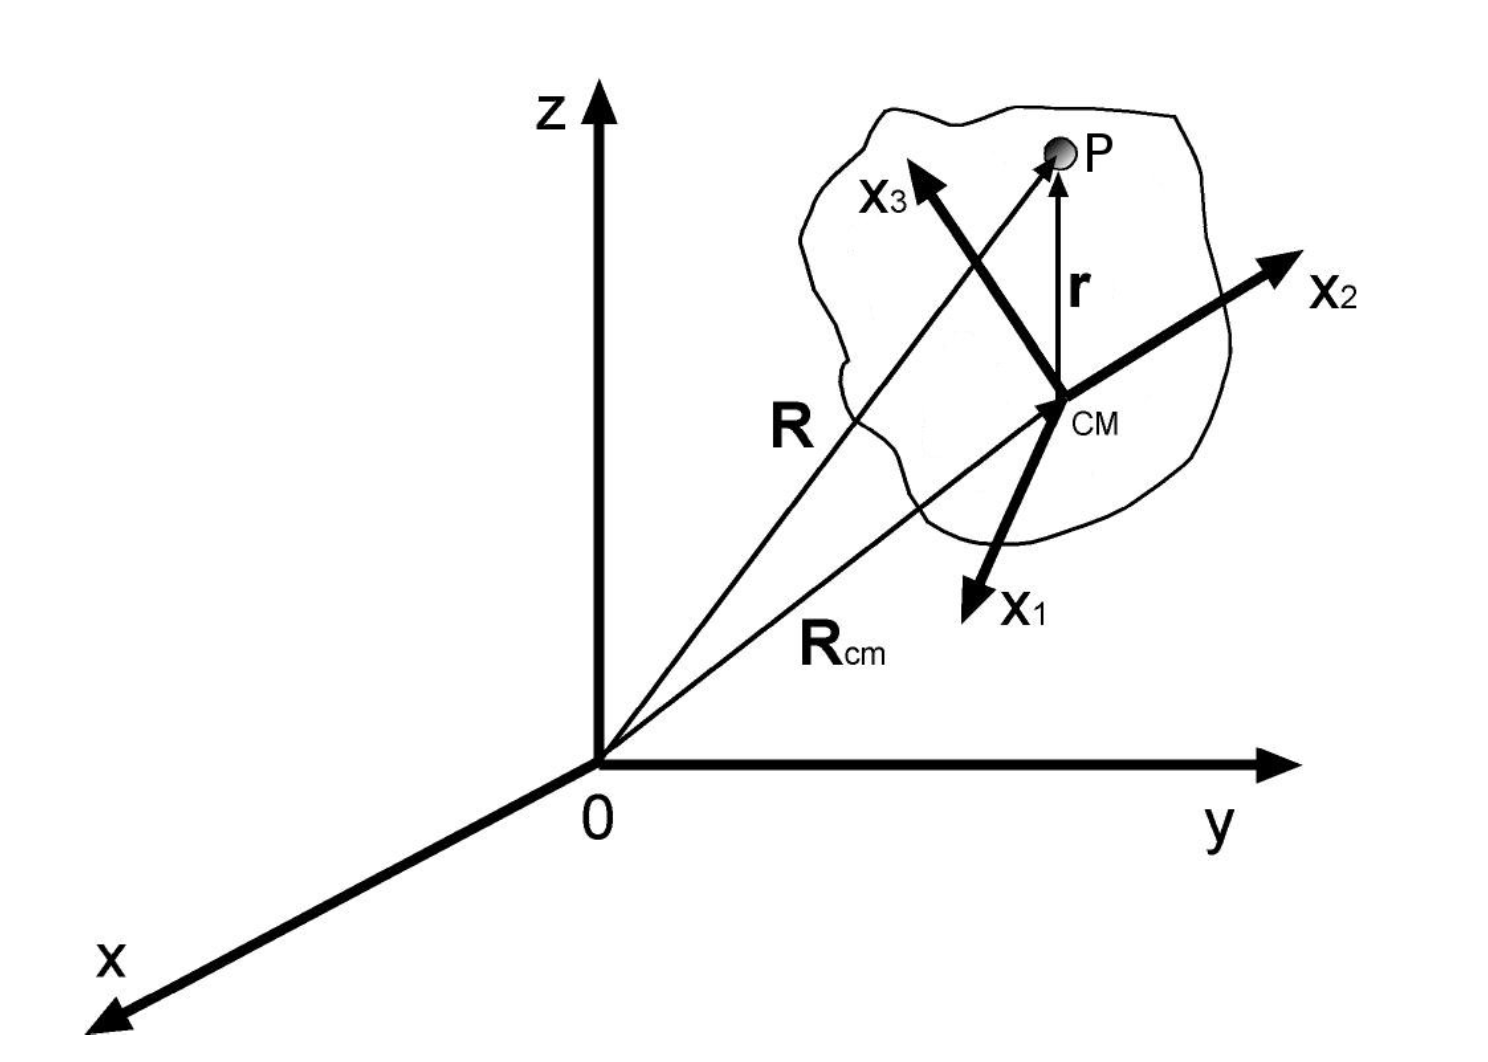
\includegraphics[width=\textwidth]{Figuras/SolidRef.png}
    \end{column}
  \end{columns}
  \uncover<4->{\begin{alertblock}{Terminología}
    \footnotesize $\Scue$ es el \textbf{sistema fijo en el cuerpo}. No es el
    ``sistema centro de masa'' usual, que solo se traslada con el CM sin rotar.
  \end{alertblock}}
\end{frame}

\begin{frame}
  \frametitle{Desplazamiento general del cuerpo rígido}
  \begin{itemize}
    \item<1-> Posición de un punto $P$ del cuerpo en $\Slab$:
          $\vect{R}=\vect{R}_{\mathrm{cm}}+\vect{r}$, con $\vect{r}$ la posición de
          $P$ respecto al CM.
    \item<2-> Un desplazamiento infinitesimal se descompone en
          \begin{itemize}
            \item \textbf{traslación} del CM, sin cambiar la orientación de $\Scue$
                  respecto a $\Slab$: $d\vect{R}_{\mathrm{cm}}$;
            \item \textbf{rotación} de $\Scue$ alrededor de un eje que pasa por el CM:
                  $d\vect{r}$.
          \end{itemize}
          \[ d\vect{R}=d\vect{R}_{\mathrm{cm}}+d\vect{r}. \]
    \item<3-> Las componentes de $\vect{r}$ en $\Scue$ son \textbf{constantes}. Visto
          desde $\Slab$, $|\vect{r}|$ es constante, de modo que
          $d(\vect{r}\cdot\vect{r})=0 \Rightarrow d\vect{r}\perp\vect{r}$:
          solo cambia la \textbf{dirección} de $\vect{r}$.
  \end{itemize}
  \begin{columns}[T]
    \begin{column}{0.68\textwidth}
      \begin{itemize}
        \item<4-> \textbf{Teorema de Euler:} todo desplazamiento de un cuerpo rígido
              con un punto fijo es una rotación alrededor de un eje que pasa por ese
              punto.
      \end{itemize}
    \end{column}
    \begin{column}{0.30\textwidth}
      \centering
      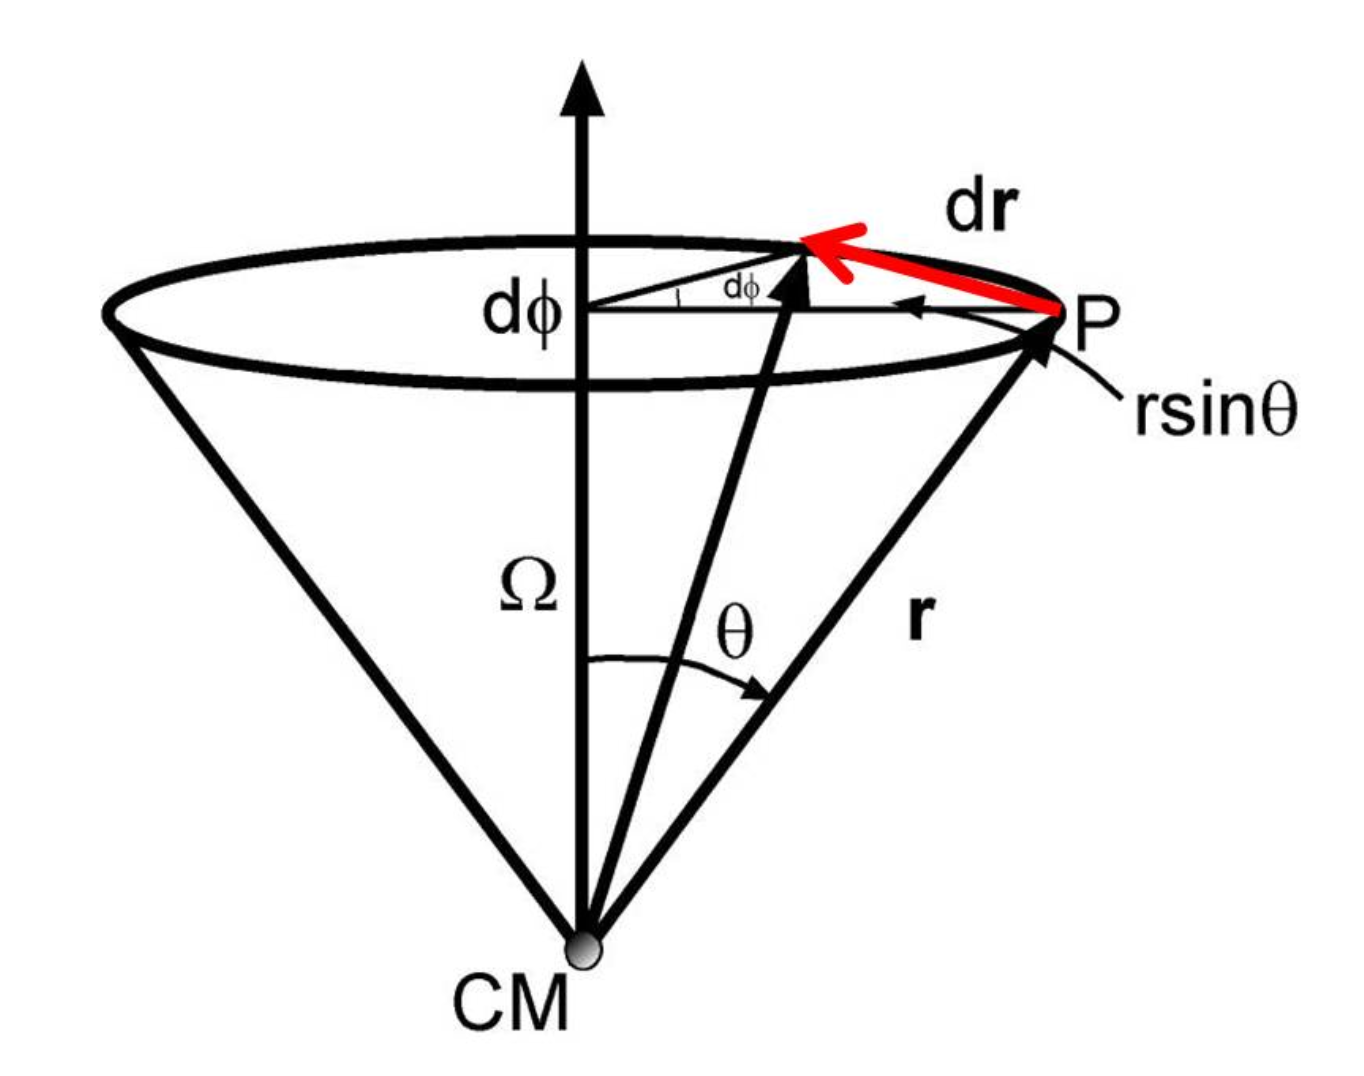
\includegraphics[width=\textwidth]{Figuras/Infinitesimal.png}
    \end{column}
  \end{columns}
\end{frame}

\begin{frame}
  \frametitle{Rotación infinitesimal y velocidad angular}
  \begin{columns}[T]
    \begin{column}{0.60\textwidth}
      \begin{itemize}
        \item<1-> Sea $\dPhi$ la rotación infinitesimal: módulo $d\Phi$ (ángulo girado),
              dirección dada por la regla de la mano derecha.
        \item<2-> Si $\alpha$ es el ángulo entre $\dPhi$ y $\vect{r}$:
              $|d\vect{r}|=(r\sen\alpha)\,d\Phi$, y $d\vect{r}\perp(\dPhi,\vect{r})$.
              Módulo y dirección: $d\vect{r}=\dPhi\times\vect{r}$.
        \item<3-> Dividiendo por $dt$:
              \[ \vect{v}=\vect{v}_{\mathrm{cm}}+\bOmega\times\vect{r},
                 \qquad \bOmega\equiv\frac{\dPhi}{dt}. \]
      \end{itemize}
    \end{column}
    \begin{column}{0.38\textwidth}
      \centering
      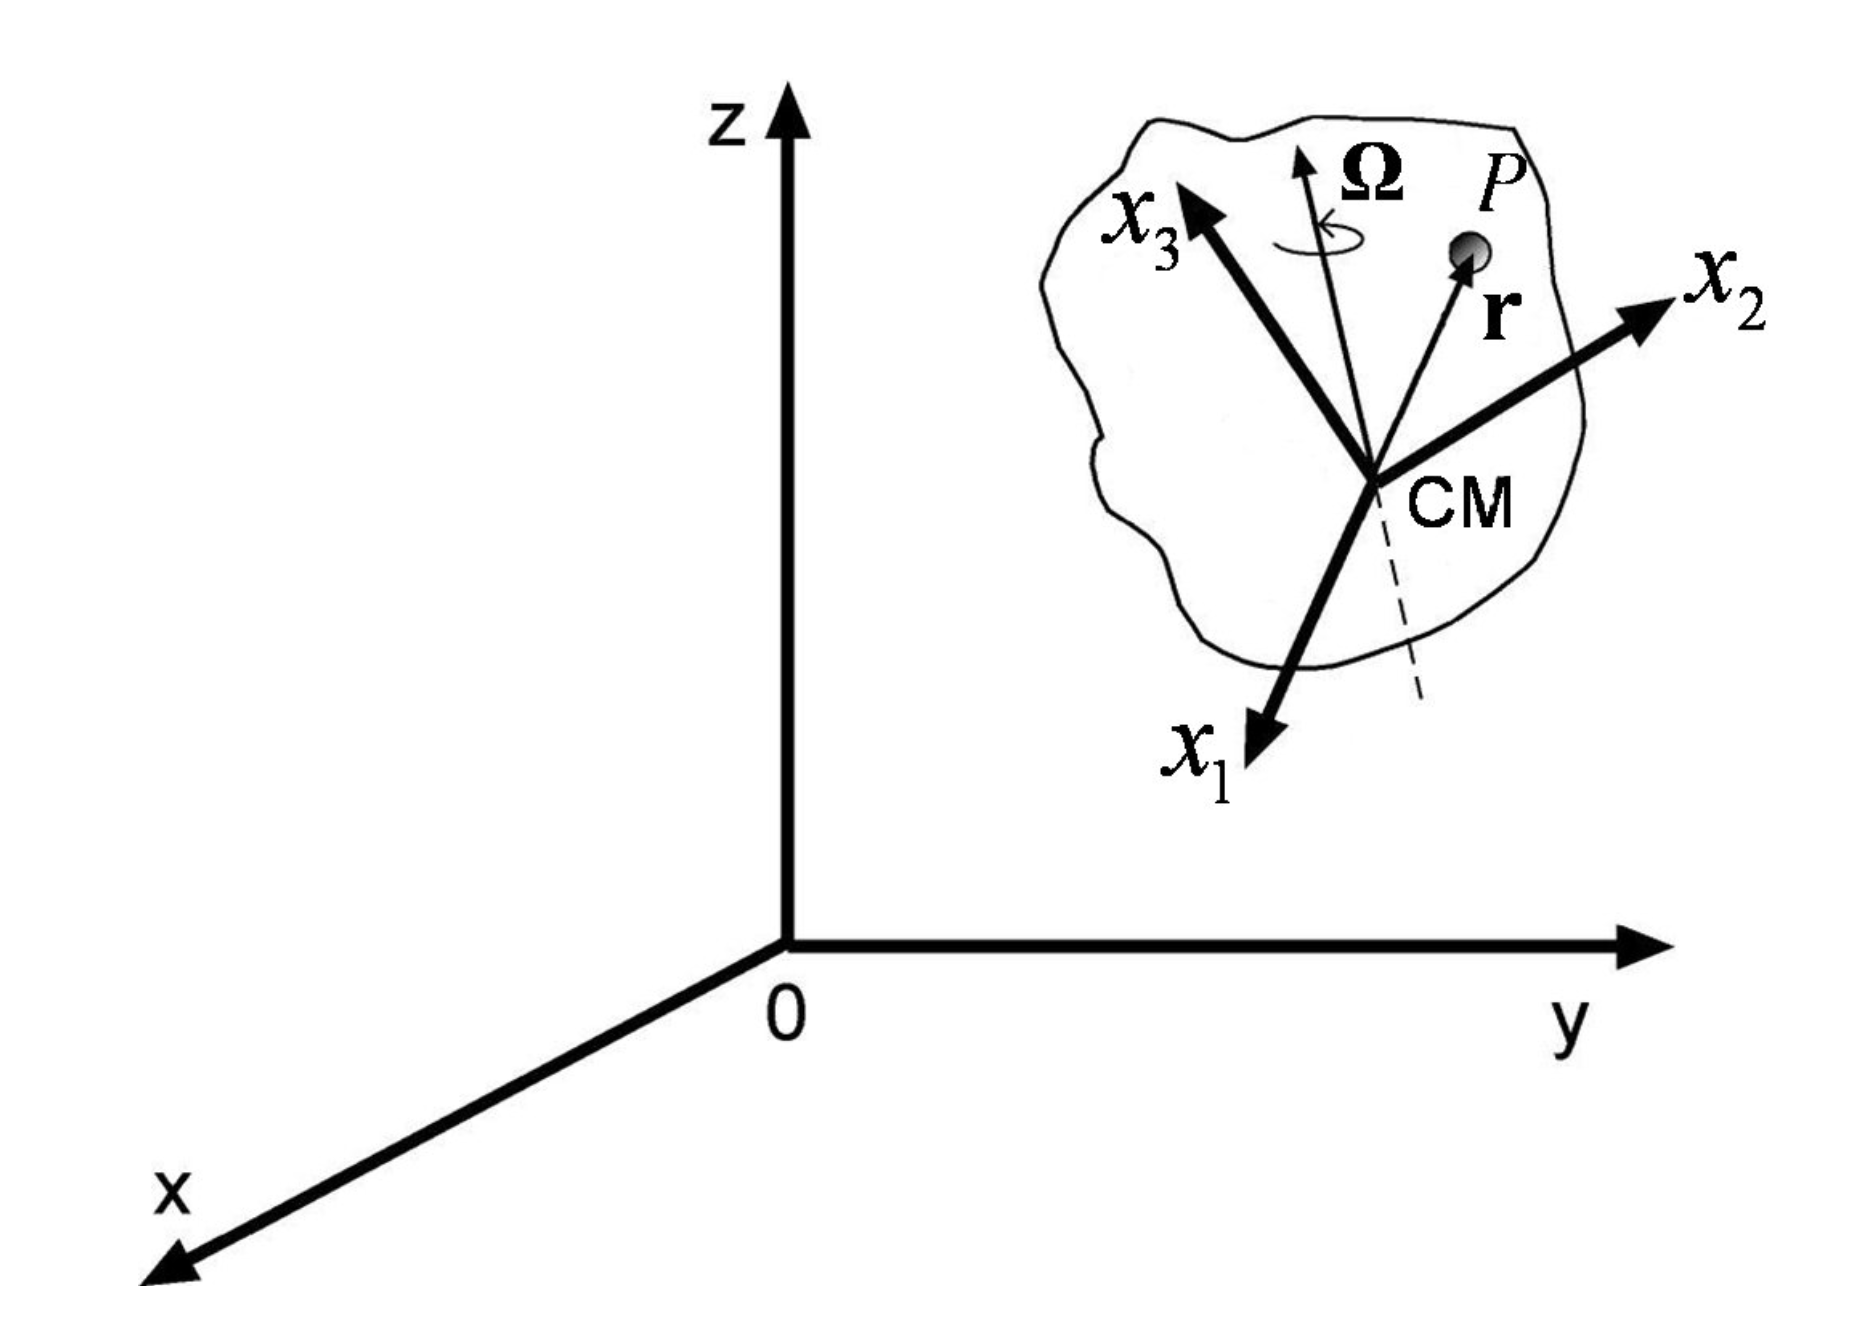
\includegraphics[width=\textwidth]{Figuras/VelocidadP.png}
    \end{column}
  \end{columns}
  \begin{itemize}
    \item<4-> $\vect{v}=d\vect{R}/dt$ (velocidad de $P$ en $\Slab$),
          $\vect{v}_{\mathrm{cm}}=d\vect{R}_{\mathrm{cm}}/dt$,
          $\bOmega$: velocidad angular instantánea, $[\Omega]=\mathrm{s}^{-1}$.
    \item<5-> $\bOmega$ es \textbf{la misma para todo el cuerpo}; puede cambiar en el
          tiempo. Para los ejes del cuerpo, $d\uv{x}_i/dt=\bOmega\times\uv{x}_i$.
  \end{itemize}
\end{frame}

% =====================================================================
\section{Rotaciones y el grupo SO(3)}
% =====================================================================

\begin{frame}
  \frametitle{Notación de esta clase}
  \begin{itemize}
    \item<1-> Bases ortonormales: $\{\uv{x},\uv{y},\uv{z}\}$ de $\Slab$ y
          $\{\uv{x}_1,\uv{x}_2,\uv{x}_3\}$ de $\Scue$.
    \item<2-> Un mismo vector $\vect{r}$ tiene dos columnas de componentes:
          \[
            \colLab{r}=\begin{pmatrix} r_x\\ r_y\\ r_z\end{pmatrix}\ \text{(en $\Slab$)},
            \qquad
            \colCue{r}=\begin{pmatrix} r_1\\ r_2\\ r_3\end{pmatrix}\ \text{(en $\Scue$)}.
          \]
    \item<3-> Rotación \textbf{pasiva}: el vector no cambia; giran los ejes y cambian sus
          componentes:
          \[
            \colCue{r}=\Rot\,\colLab{r}
            \quad\Longleftrightarrow\quad
            r_i=A_{ij}\,r_j ,
            \qquad
            \colLab{r}=\Rot^{\tr}\colCue{r}.
          \]
          (Suma sobre índices repetidos; los índices latinos de $\Slab$ recorren $x,y,z$.)
    \item<4-> Velocidad angular: $\Omega_x,\Omega_y,\Omega_z$ en $\Slab$ y
          $\Omega_1,\Omega_2,\Omega_3$ en $\Scue$.
  \end{itemize}
\end{frame}

\begin{frame}
  \frametitle{Rotación pasiva en el plano}
  \begin{columns}[T]
    \begin{column}{0.62\textwidth}
      \begin{itemize}
        \item<1-> Ejes girados un ángulo $\phi$ alrededor de $x_3$:
          \[
            \begin{pmatrix} x_1'\\ x_2'\end{pmatrix}
            =\underbrace{\begin{pmatrix}\cos\phi & \sen\phi\\ -\sen\phi & \cos\phi\end{pmatrix}}_{\Rot_\phi}
            \begin{pmatrix} x_1\\ x_2\end{pmatrix}.
          \]
        \item<2-> Propiedades:
          $\Rot_\phi^{\tr}=\Rot_{-\phi}=\Rot_\phi^{-1}$,\quad $\det\Rot_\phi=+1$.
        \item<3-> Composición alrededor del \textbf{mismo} eje:
          $\Rot_\phi\Rot_\gamma=\Rot_{\phi+\gamma}=\Rot_\gamma\Rot_\phi$.
      \end{itemize}
    \end{column}
    \begin{column}{0.36\textwidth}
      \centering
      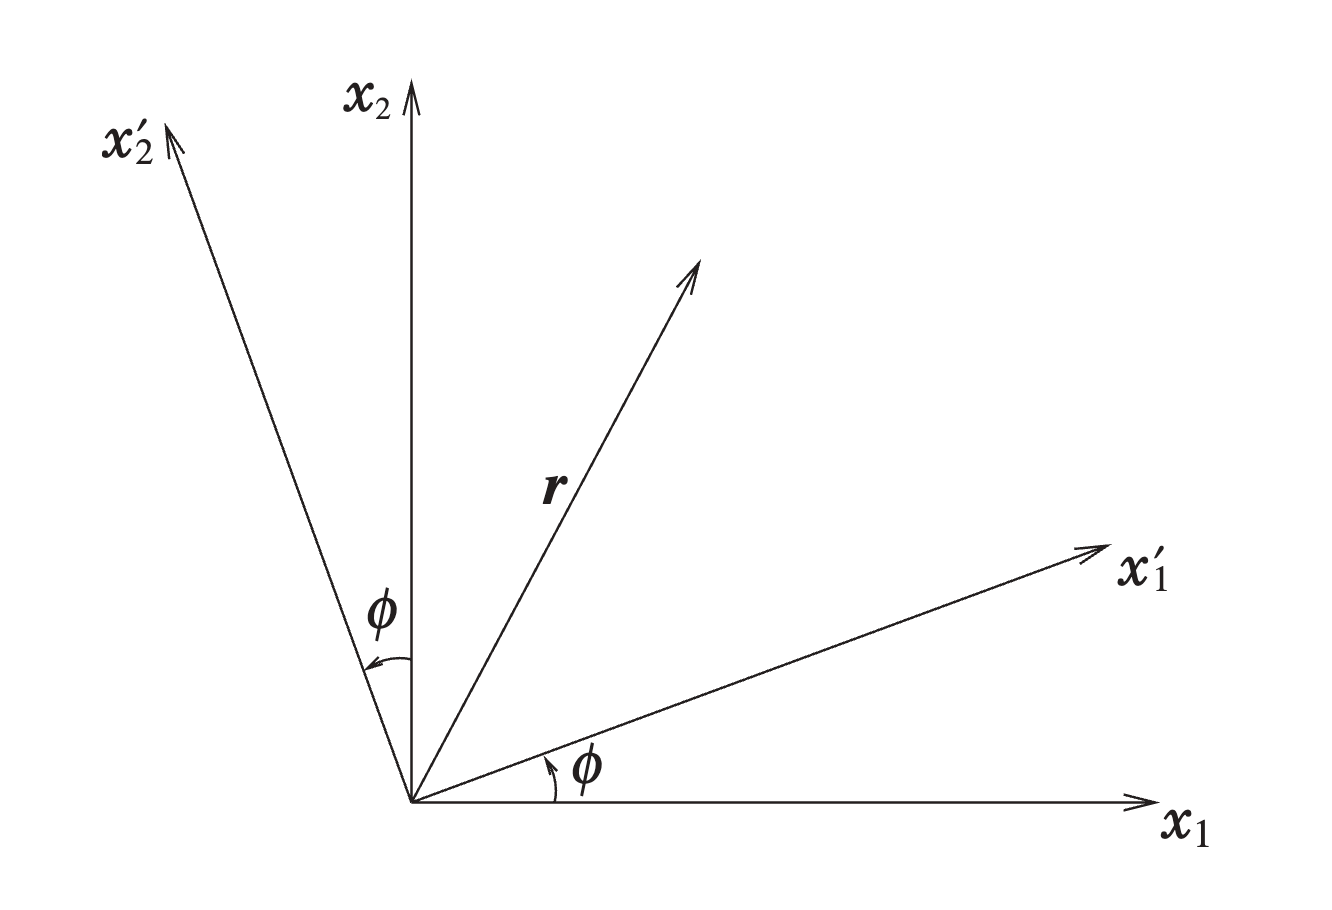
\includegraphics[width=\textwidth]{Figuras/RotacionSimple.png}
    \end{column}
  \end{columns}
  \begin{itemize}
    \item<4-> \textbf{Atención:} la rotación \emph{activa} del vector un ángulo $\phi$
          tiene la matriz transpuesta. Mezclar ambas convenciones es la fuente más
          común de errores de signo.
  \end{itemize}
\end{frame}

\begin{frame}
  \frametitle{Matrices ortogonales: los grupos O(3) y SO(3)}
  \begin{itemize}
    \item<1-> Una transformación que preserva longitudes cumple
          $\Rot^{\tr}\Rot=\Id$. Esto implica $\det\Rot=\pm1$.
    \item<2-> $\mathbf{O}(3)$: todas las matrices ortogonales reales. Incluye
          reflexiones e inversiones ($\det=-1$).
    \item<3-> Las \textbf{rotaciones propias} ($\det=+1$) forman el subgrupo
          $\mathbf{SO}(3)$:
      \begin{itemize}
        \item \textbf{Cerradura:} $\Rot,\mathbb{B}\in\mathbf{SO}(3)\Rightarrow\Rot\mathbb{B}\in\mathbf{SO}(3)$.
        \item \textbf{Asociatividad:} $(\Rot\mathbb{B})\mathbb{C}=\Rot(\mathbb{B}\mathbb{C})$.
        \item \textbf{Neutro:} $\Id\,\Rot=\Rot\,\Id=\Rot$.
        \item \textbf{Inverso:} $\Rot^{-1}=\Rot^{\tr}\in\mathbf{SO}(3)$.
      \end{itemize}
    \item<4-> En 3D el grupo \textbf{no es conmutativo}: $\Rot\mathbb{B}\neq\mathbb{B}\Rot$
          en general (el libro de la motivación).
    \item<5-> \textbf{Conteo de parámetros:} 9 elementos $-$ 6 condiciones
          independientes en $\Rot^{\tr}\Rot=\Id$ $=$ \textbf{3 parámetros}: los tres
          grados de libertad de orientación.
    \item<6-> Las rotaciones son matrices \emph{ortogonales}. ``Unitario'' es la
          generalización a matrices complejas.
  \end{itemize}
\end{frame}

% =====================================================================
\section{Ángulos de Euler}
% =====================================================================

\begin{frame}
  \frametitle{Precesión, nutación y rotación propia}
  \begin{columns}[T]
    \begin{column}{0.66\textwidth}
      \begin{itemize}
        \item<1-> Tres movimientos característicos de un trompo:
          \textbf{precesión} (giro alrededor de un eje fijo en $\Slab$),
          \textbf{nutación} (inclinación respecto a ese eje) y
          \textbf{rotación propia} (giro del cuerpo sobre su eje).
        \item<2-> \textbf{Línea nodal} $\uv{N}$: intersección de los planos
              $(x,y)$ y $(x_1,x_2)$; $\uv{N}\perp\uv{z}$ y $\uv{N}\perp\uv{x}_3$.
      \end{itemize}
    \end{column}
    \begin{column}{0.32\textwidth}
      \centering
      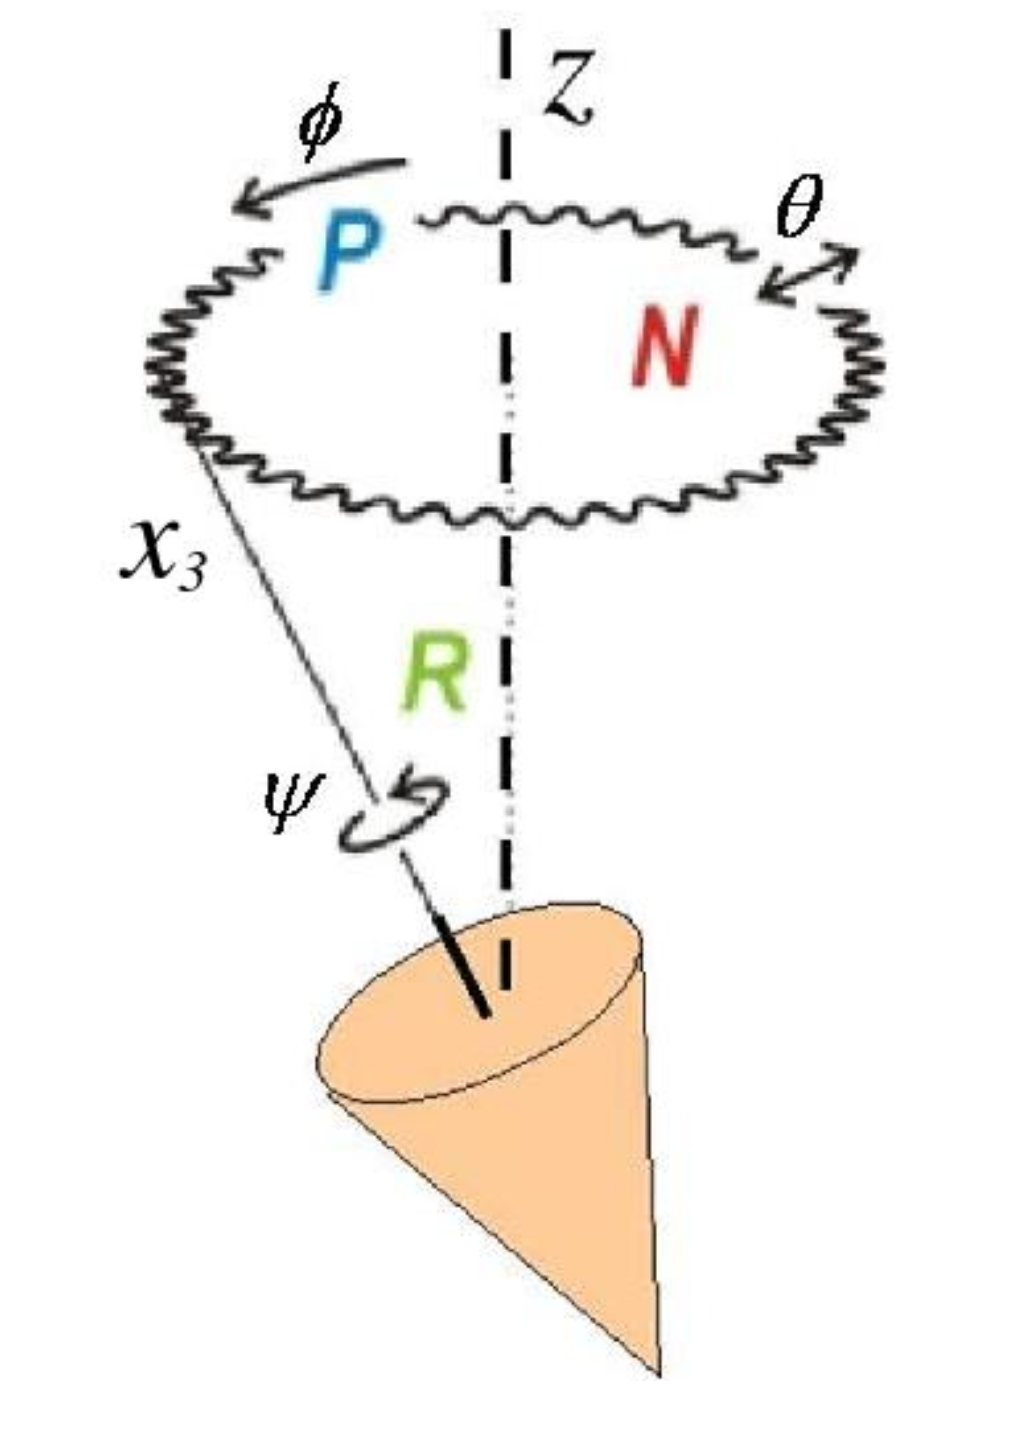
\includegraphics[width=0.9\textwidth]{Figuras/PrecesionNutacion.png}
    \end{column}
  \end{columns}
  \begin{itemize}
    \item<3-> \textbf{Ángulo de precesión} $\phi\in[0,2\pi)$: giro alrededor de $z$,
          en el plano $(x,y)$, medido desde $x$ hasta $\uv{N}$.
    \item<4-> \textbf{Ángulo de nutación} $\theta\in[0,\pi]$: giro alrededor de
          $\uv{N}$, medido desde $z$ hasta $x_3$.
    \item<5-> \textbf{Ángulo de rotación propia} $\psi\in[0,2\pi)$: giro alrededor de
          $x_3$, en el plano $(x_1,x_2)$, medido desde $\uv{N}$ hasta $x_1$.
  \end{itemize}
\end{frame}

\begin{frame}
  \frametitle{Tres rotaciones sucesivas (convención $z$–$x$–$z$)}
  \begin{itemize}
    \item<1-> Hacemos coincidir los orígenes $O$ y CM y llevamos $\Slab$ hasta $\Scue$
          con tres rotaciones pasivas:
          \[
            \Slab \xrightarrow[\text{eje } z]{\ \phi\ } \Slab'
                  \xrightarrow[\text{eje } x'=\uv{N}]{\ \theta\ } \Slab''
                  \xrightarrow[\text{eje } x_3''=x_3]{\ \psi\ } \Scue .
          \]
  \end{itemize}
  \centering
  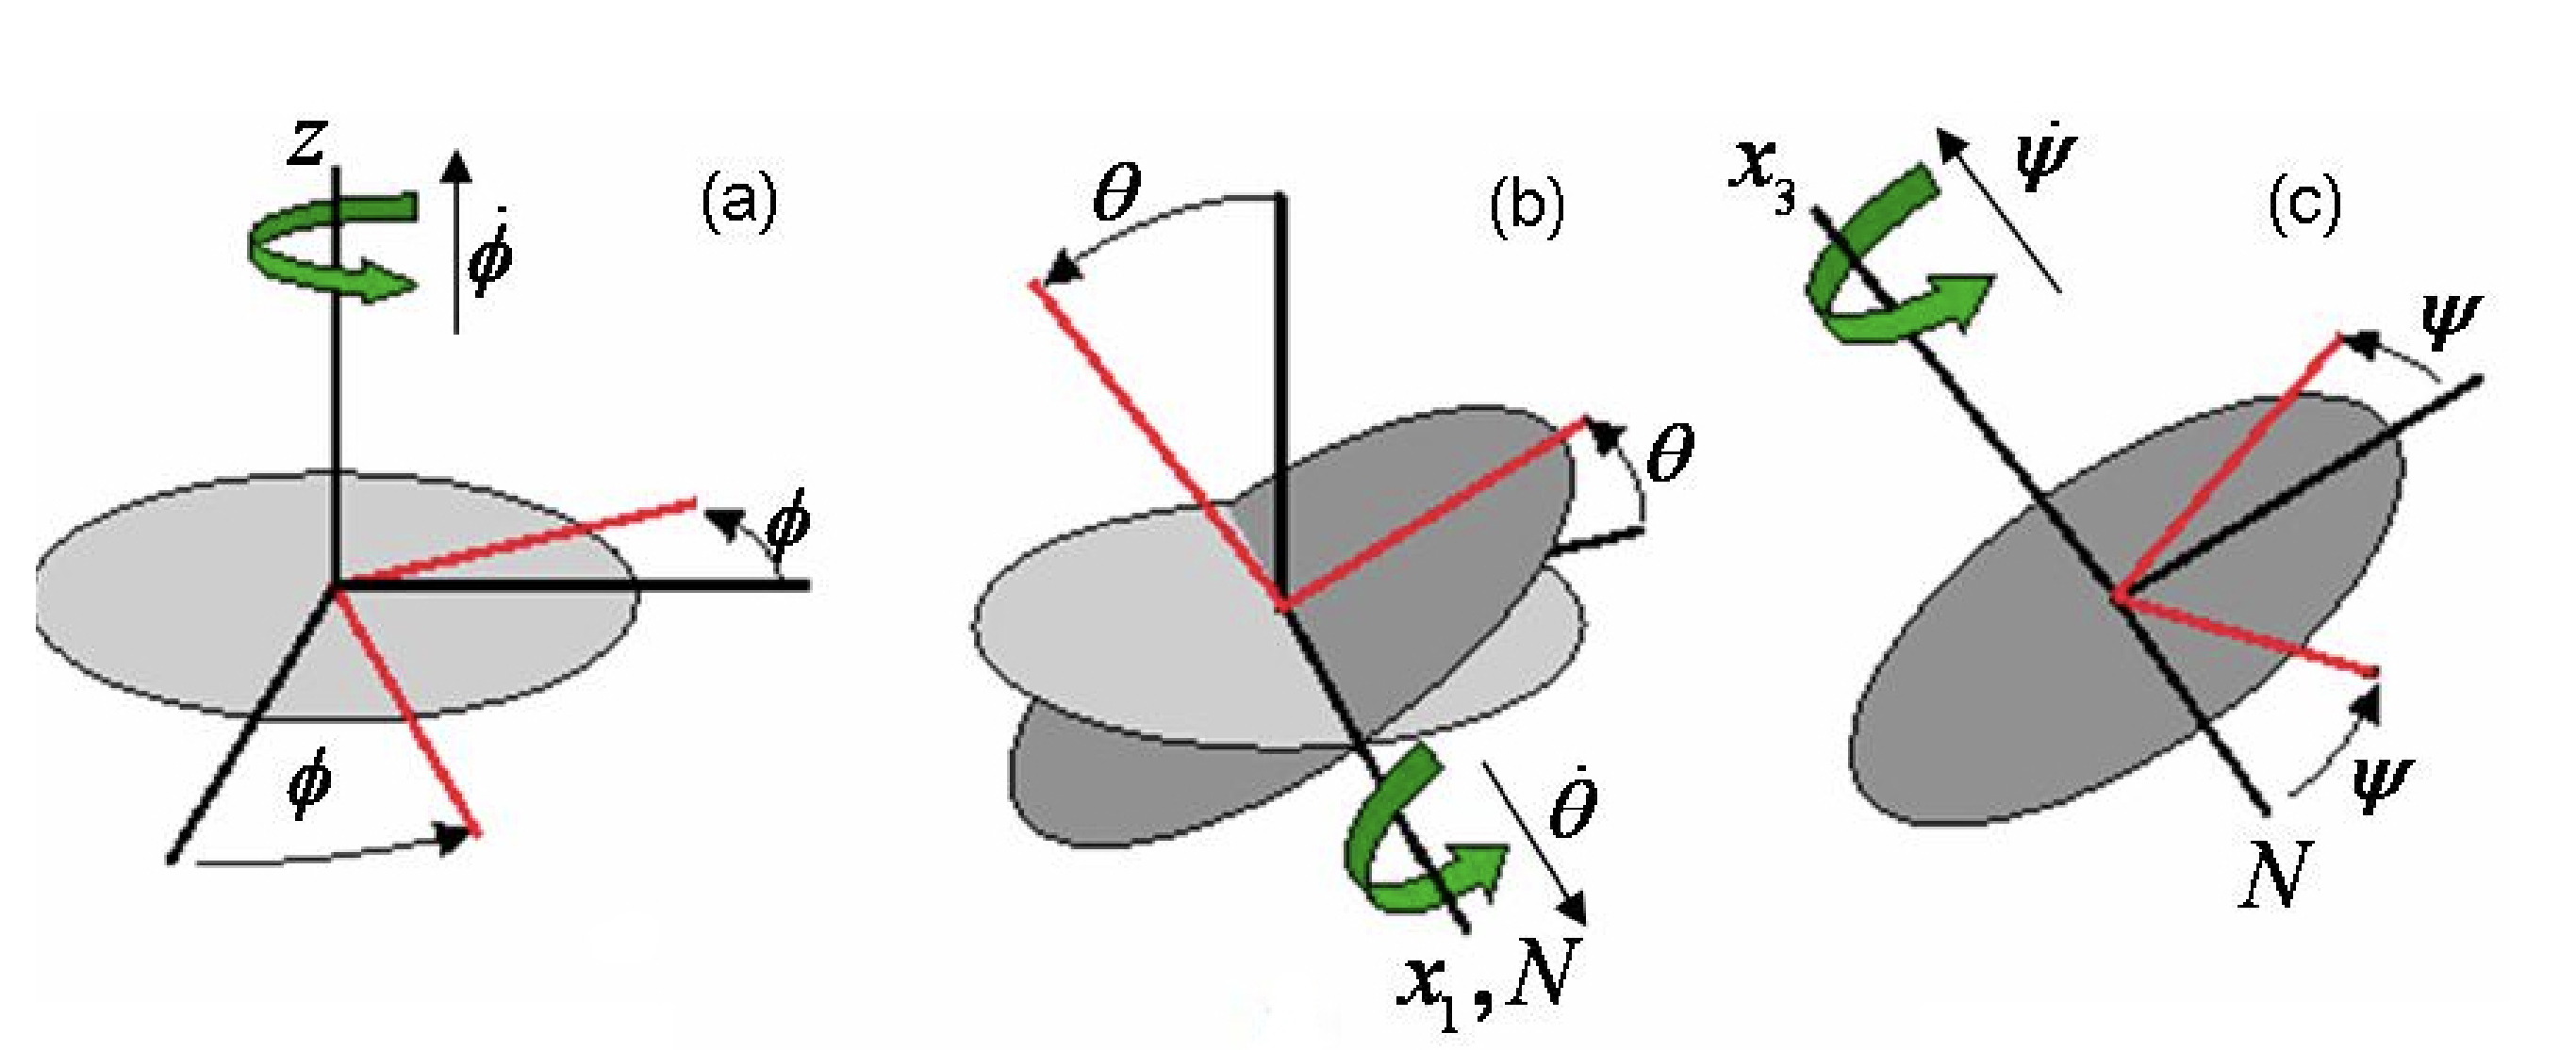
\includegraphics[width=1.7in]{Figuras/RotacionesEuler.png}
  \uncover<2->{%
  {\scriptsize
  \[
    \Rot_\phi=\begin{pmatrix}\cos\phi&\sen\phi&0\\-\sen\phi&\cos\phi&0\\0&0&1\end{pmatrix},\
    \Rot_\theta=\begin{pmatrix}1&0&0\\0&\cos\theta&\sen\theta\\0&-\sen\theta&\cos\theta\end{pmatrix},\
    \Rot_\psi=\begin{pmatrix}\cos\psi&\sen\psi&0\\-\sen\psi&\cos\psi&0\\0&0&1\end{pmatrix}
  \]}}
  \begin{itemize}
    \item<3-> Cada matriz actúa sobre las componentes del sistema intermedio
          anterior; la primera rotación queda \textbf{a la derecha}:
          $\colCue{r}=\Rot_\psi\Rot_\theta\Rot_\phi\,\colLab{r}$.
  \end{itemize}
\end{frame}

\begin{frame}
  \frametitle{La matriz de Euler}
  \begin{itemize}
    \item<1-> Componiendo las tres rotaciones, $\Rot\equiv\Rot_\psi\Rot_\theta\Rot_\phi$:
  \end{itemize}
  {\scriptsize
  \[
    \Rot=\begin{pmatrix}
      \cos\psi\cos\phi-\cos\theta\sen\phi\sen\psi &
      \cos\psi\sen\phi+\cos\theta\cos\phi\sen\psi &
      \sen\psi\sen\theta\\[2pt]
      -\sen\psi\cos\phi-\cos\theta\sen\phi\cos\psi &
      -\sen\psi\sen\phi+\cos\theta\cos\phi\cos\psi &
      \cos\psi\sen\theta\\[2pt]
      \sen\theta\sen\phi & -\sen\theta\cos\phi & \cos\theta
    \end{pmatrix}
  \]}
  \begin{itemize}
    \item<2-> Inversa: como cada factor es ortogonal,
          \[
            \Rot^{-1}=\Rot^{\tr}
            =\Rot_\phi^{\tr}\Rot_\theta^{\tr}\Rot_\psi^{\tr}
            =\Rot_{-\phi}\,\Rot_{-\theta}\,\Rot_{-\psi}.
          \]
          La inversa de un producto invierte el orden de los factores.
    \item<3-> $\Rot^{\tr}$ es la transpuesta de la matriz de arriba: lleva componentes de
          $\Scue$ a $\Slab$, $\colLab{r}=\Rot^{\tr}\colCue{r}$.
    \item<4-> \textbf{Verificaciones mínimas:} $\Rot^{\tr}\Rot=\Id$, $\det\Rot=+1$,
          $\Rot(\phi,0,0)=\Rot_\phi$, $\Rot(0,\theta,0)=\Rot_\theta$.
  \end{itemize}
\end{frame}

\begin{frame}
  \frametitle{Cosenos directores: cómo leer la matriz $\Rot$}
  \begin{itemize}
    \item<1-> Como $r_i=\uv{x}_i\cdot\vect{r}$ y $\vect{r}=r_x\uv{x}+r_y\uv{y}+r_z\uv{z}$,
          los elementos de $\Rot$ son productos escalares:
          \[
            A_{ij}=\uv{x}_i\cdot\uv{e}_j,\qquad \uv{e}_j\in\{\uv{x},\uv{y},\uv{z}\}.
          \]
    \item<2-> \textbf{Fila $i$} de $\Rot$ = componentes de $\uv{x}_i$ (eje del cuerpo)
          en $\Slab$. Por ejemplo:
          \[ \uv{x}_3=\sen\theta\sen\phi\,\uv{x}-\sen\theta\cos\phi\,\uv{y}+\cos\theta\,\uv{z}. \]
    \item<3-> \textbf{Columna $j$} de $\Rot$ = componentes de $\uv{e}_j$ (eje del
          laboratorio) en $\Scue$. Por ejemplo:
          \[ \uv{z}=\sen\theta\sen\psi\,\uv{x}_1+\sen\theta\cos\psi\,\uv{x}_2+\cos\theta\,\uv{x}_3. \]
    \item<4-> \textbf{Lectura física:} $\uv{x}_3$ en $\Slab$ no depende de $\psi$,
          porque girar alrededor de $x_3$ no mueve a $x_3$. Del mismo modo,
          $\uv{z}$ en $\Scue$ no depende de $\phi$.
    \item<5-> Las filas (y las columnas) son ortonormales: esa es exactamente la
          condición $\Rot\Rot^{\tr}=\Rot^{\tr}\Rot=\Id$.
  \end{itemize}
\end{frame}

\begin{frame}
  \frametitle{Dominio de validez: la singularidad en $\theta=0,\pi$}
  \begin{itemize}
    \item<1-> Si $\theta=0$, entonces $\Rot_\theta=\Id$ y
          $\Rot=\Rot_\psi\Rot_\phi=\Rot_{\phi+\psi}$.
          Solo la suma $\phi+\psi$ tiene significado (para $\theta=\pi$, solo la
          diferencia $\phi-\psi$).
    \item<2-> La línea nodal $\uv{N}$ no está definida: $x_3$ coincide con $\pm z$.
    \item<3-> El mapa $(\phi,\theta,\psi)\mapsto\Rot$ es regular solo para
          $0<\theta<\pi$. Ninguna parametrización con tres ángulos cubre
          $\mathbf{SO}(3)$ sin singularidades (\emph{gimbal lock}).
    \item<4-> \textbf{Consecuencias prácticas:}
      \begin{itemize}
        \item elegir el eje $z$ de modo que el movimiento de interés tenga $\theta$
              lejos de $0$ y $\pi$ (en un trompo pesado, $z$ vertical);
        \item en simulaciones numéricas, integrar directamente $\Rot(t)$ o usar
              cuaterniones cuando $\theta$ se acerca a $0$ o $\pi$.
      \end{itemize}
  \end{itemize}
\end{frame}

% =====================================================================
\section{Velocidad angular en ángulos de Euler}
% =====================================================================

\begin{frame}
  \frametitle{$\bOmega$ como suma de tres rotaciones}
  \centering
  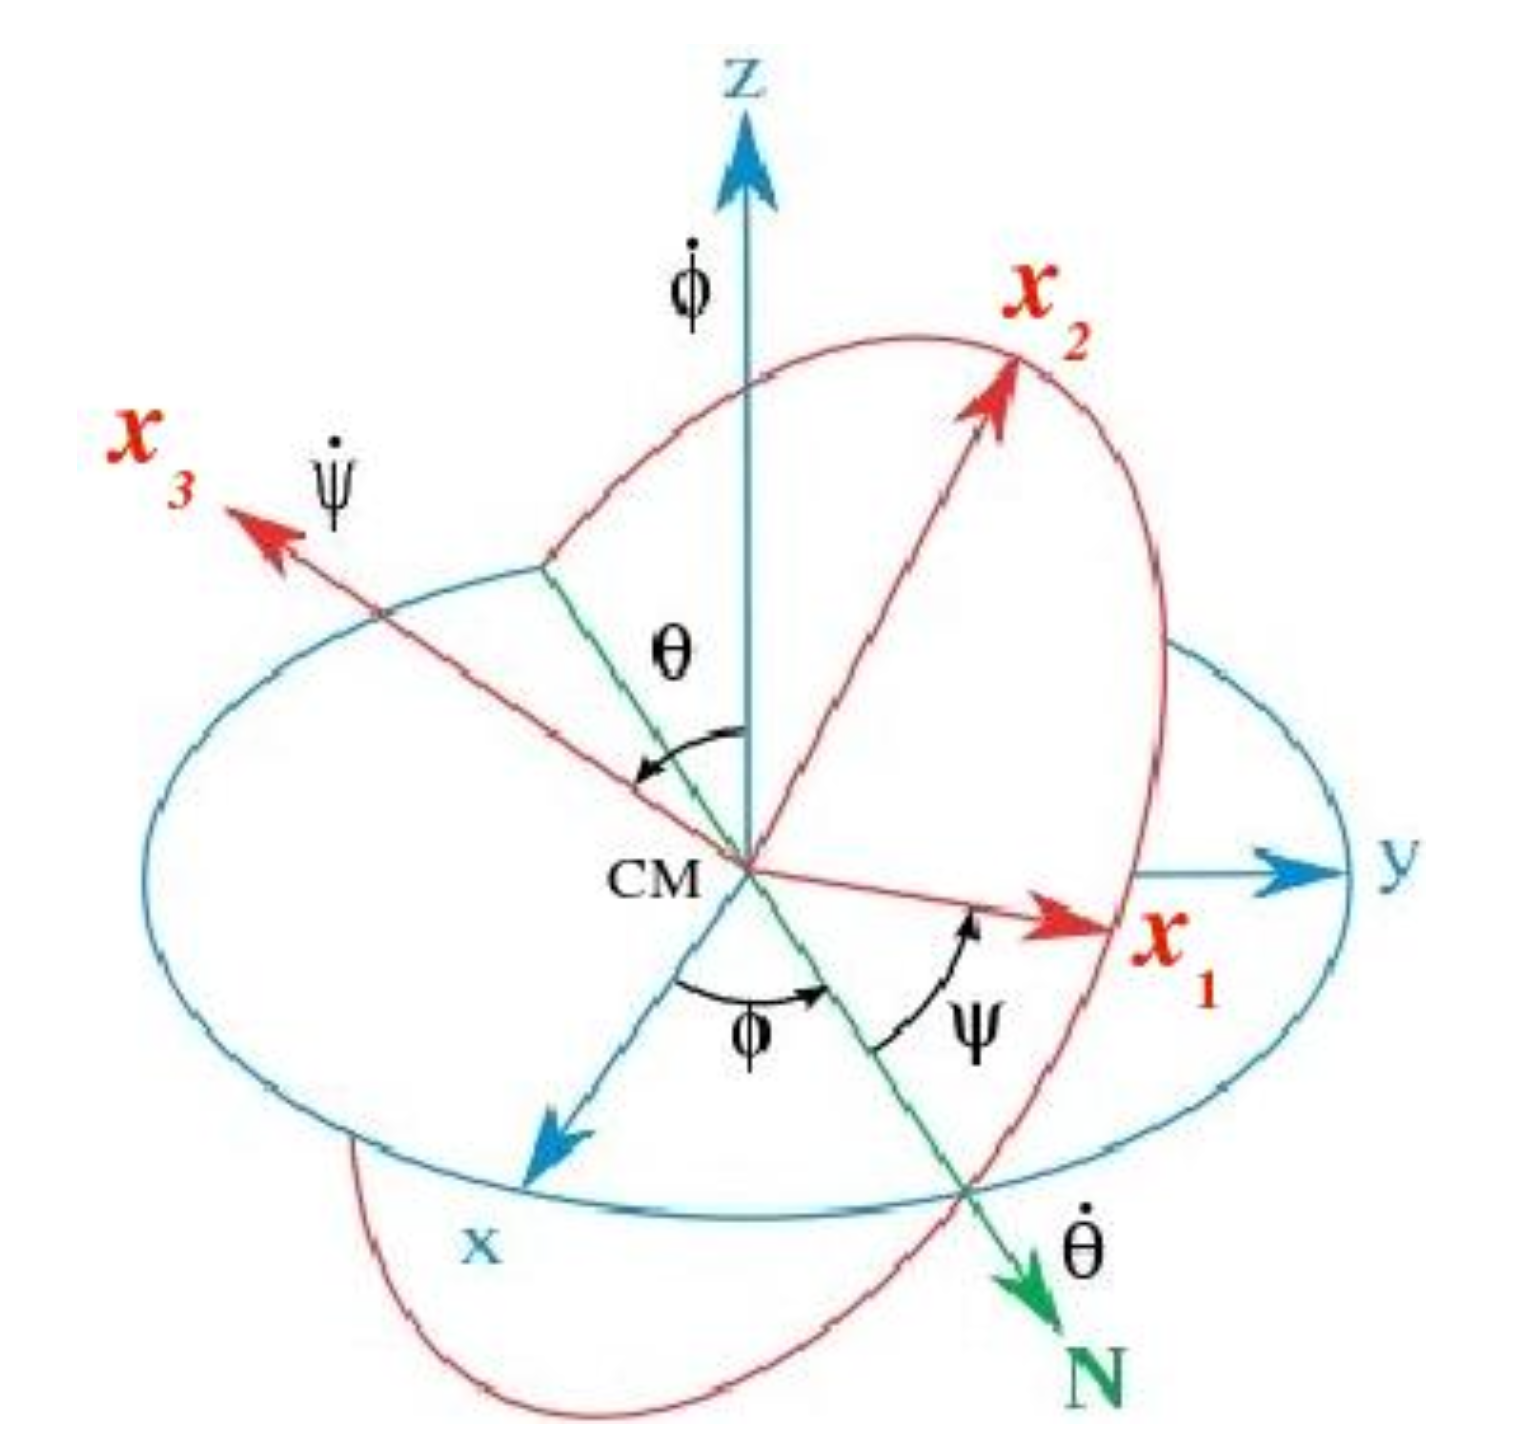
\includegraphics[height=0.95in]{Figuras/VelocidadesEuler.png}\hspace{1em}
  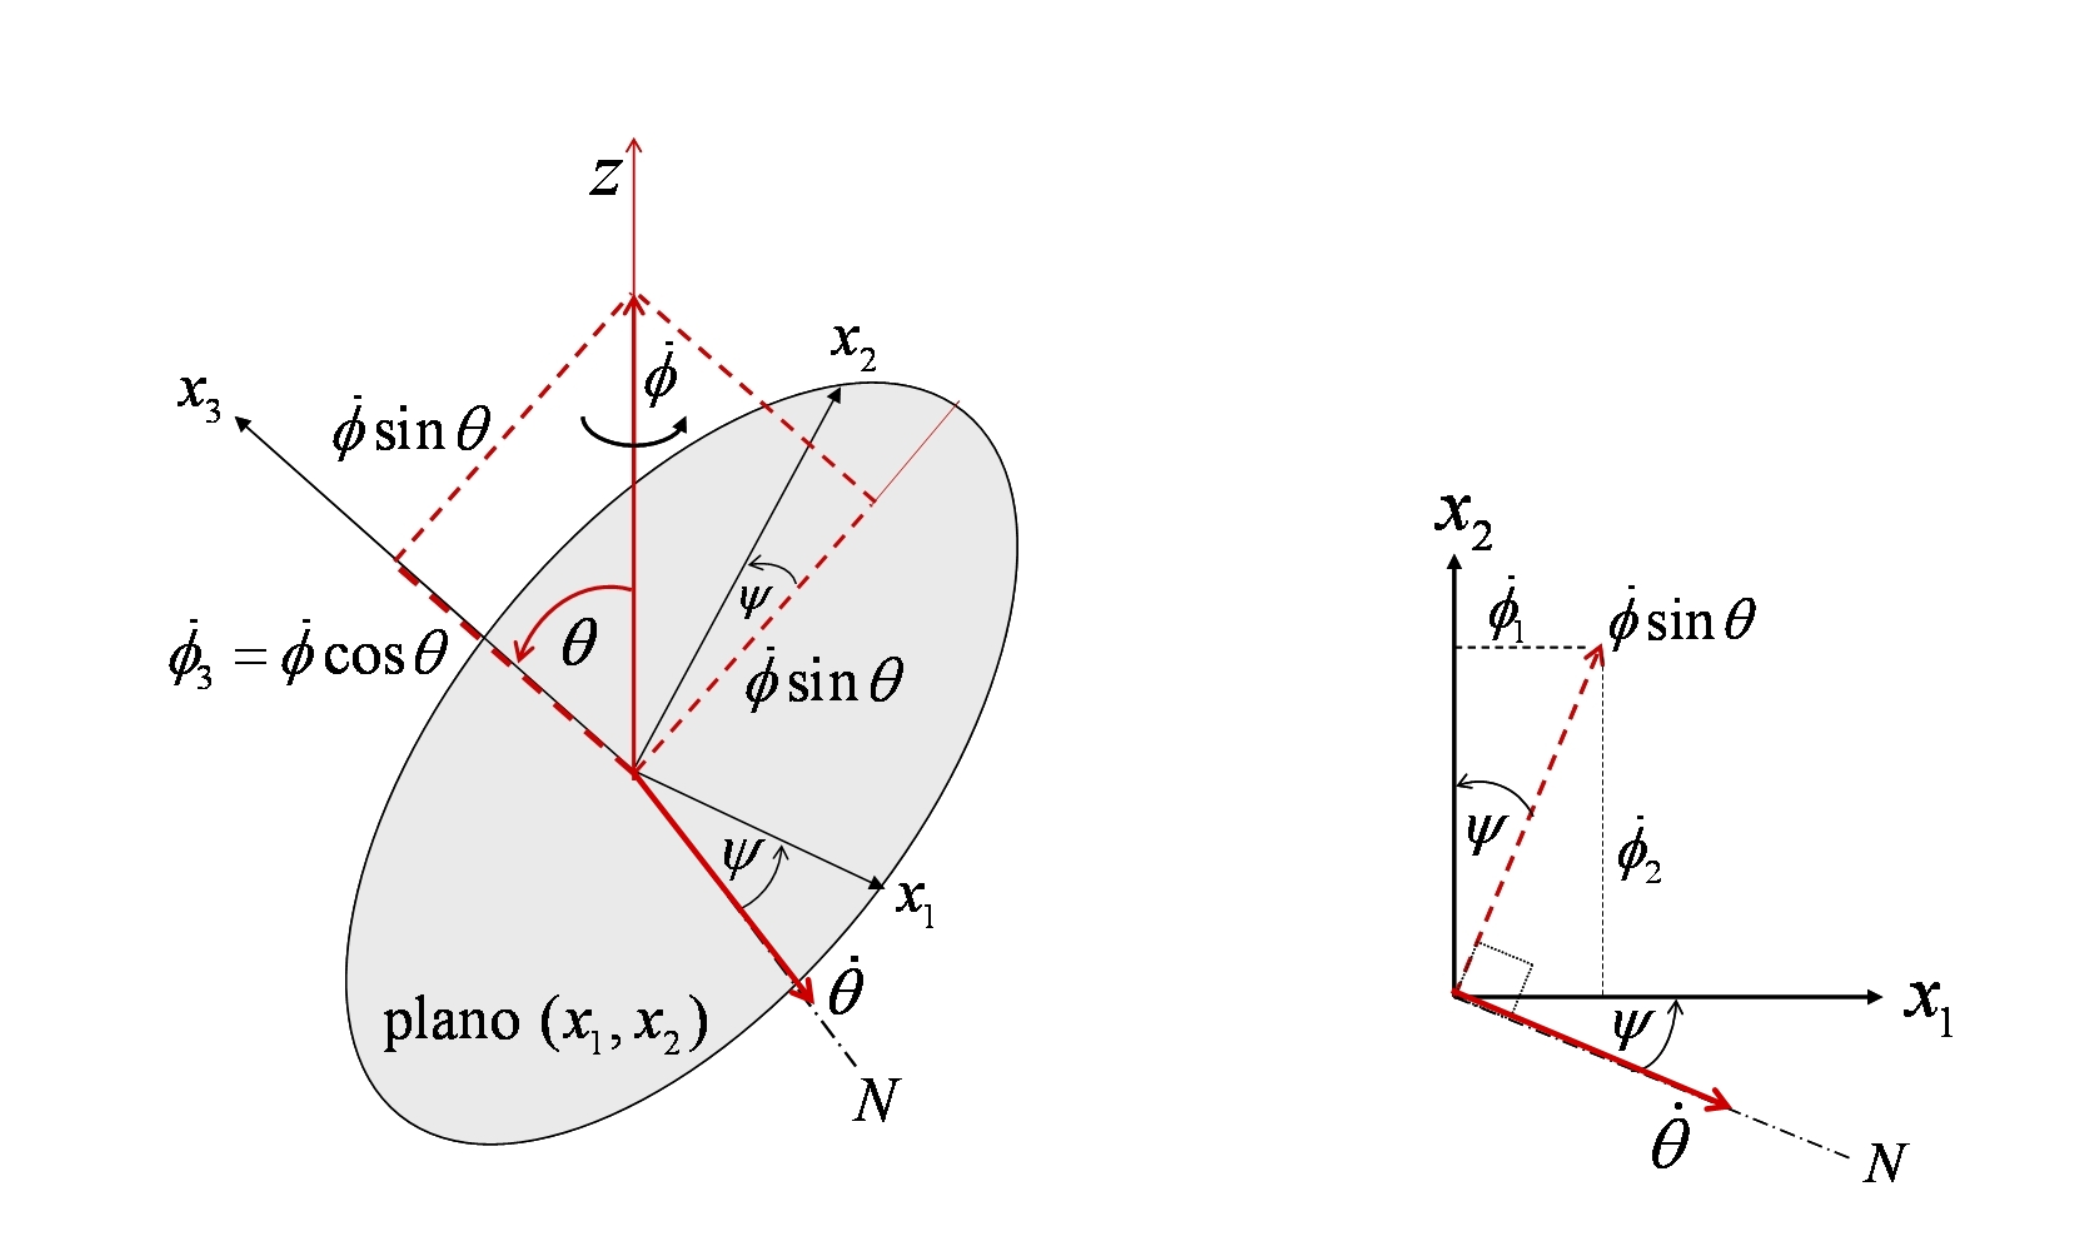
\includegraphics[height=0.95in]{Figuras/ComponentesVelocidades.png}
  \begin{itemize}
    \item<1-> Las rotaciones infinitesimales se suman como vectores. Cada ritmo
          angular apunta según su eje de giro (mano derecha):
          \[
            \bOmega=\dot\phi\,\uv{z}+\dot\theta\,\uv{N}+\dot\psi\,\uv{x}_3 .
          \]
    \item<2-> \textbf{La base $\{\uv{z},\uv{N},\uv{x}_3\}$ no es ortogonal:}
          $\uv{z}\cdot\uv{N}=\uv{N}\cdot\uv{x}_3=0$, pero
          $\uv{z}\cdot\uv{x}_3=\cos\theta$.
    \item<3-> Por eso $(\dot\phi,\dot\theta,\dot\psi)$ \textbf{no son} las componentes
          de $\bOmega$ en ninguna base ortonormal, y
          \[
            |\bOmega|^2=\dot\phi^2+\dot\theta^2+\dot\psi^2+2\dot\phi\dot\psi\cos\theta .
          \]
    \item<4-> Para obtener $\Omega_i$ o $\Omega_x,\Omega_y,\Omega_z$ basta proyectar
          $\uv{z}$, $\uv{N}$ y $\uv{x}_3$ en la base deseada. La matriz $\Rot$
          ya contiene esas proyecciones.
  \end{itemize}
\end{frame}

\begin{frame}
  \frametitle{Componentes de $\bOmega$ en el sistema del cuerpo $\Scue$}
  \begin{itemize}
    \item<1-> Proyecciones sobre $(x_1,x_2,x_3)$:
      \begin{itemize}
        \item $\uv{x}_3=(0,\,0,\,1)$: \quad $\dot\psi$ aporta solo a la tercera componente.
        \item $\uv{N}=(\cos\psi,\,-\sen\psi,\,0)$: \quad $\uv{N}\perp x_3$ y forma
              el ángulo $\psi$ con $x_1$.
        \item $\uv{z}=(\sen\theta\sen\psi,\,\sen\theta\cos\psi,\,\cos\theta)$:
              \quad tercera columna de $\Rot$.
      \end{itemize}
    \item<2-> Sumando $\dot\phi\,\uv{z}+\dot\theta\,\uv{N}+\dot\psi\,\uv{x}_3$
          componente a componente:
  \end{itemize}
  \uncover<2->{%
  \begin{block}{Velocidad angular en el sistema del cuerpo}
    \[
      \begin{aligned}
        \Omega_1 &= \dot\phi\,\sen\theta\sen\psi+\dot\theta\cos\psi\\
        \Omega_2 &= \dot\phi\,\sen\theta\cos\psi-\dot\theta\sen\psi\\
        \Omega_3 &= \dot\psi+\dot\phi\cos\theta
      \end{aligned}
    \]
  \end{block}}
  \begin{itemize}
    \item<3-> Estas son las componentes que entrarán en
          $T=\tfrac12\left(I_1\Omega_1^2+I_2\Omega_2^2+I_3\Omega_3^2\right)$
          cuando $\Scue$ son ejes principales, y en las ecuaciones de Euler.
  \end{itemize}
\end{frame}

\begin{frame}
  \frametitle{Componentes de $\bOmega$ en el laboratorio $\Slab$}
  \begin{itemize}
    \item<1-> Proyecciones sobre $(x,y,z)$:
      \begin{itemize}
        \item $\uv{z}=(0,\,0,\,1)$;
        \item $\uv{N}=(\cos\phi,\,\sen\phi,\,0)$: \quad está en el plano $(x,y)$, a un
              ángulo $\phi$ de $x$;
        \item $\uv{x}_3=(\sen\theta\sen\phi,\,-\sen\theta\cos\phi,\,\cos\theta)$:
              \quad tercera fila de $\Rot$.
      \end{itemize}
  \end{itemize}
  \uncover<2->{%
  \begin{block}{Velocidad angular en el laboratorio}
    \[
      \begin{aligned}
        \Omega_x &= \dot\theta\cos\phi+\dot\psi\,\sen\theta\sen\phi\\
        \Omega_y &= \dot\theta\sen\phi-\dot\psi\,\sen\theta\cos\phi\\
        \Omega_z &= \dot\phi+\dot\psi\cos\theta
      \end{aligned}
    \]
  \end{block}}
  \begin{itemize}
    \item<3-> \textbf{Segundo camino:} $\colLab{\Omega}=\Rot^{\tr}\colCue{\Omega}$.
          Multiplicar la transpuesta de la matriz de Euler por la columna
          $(\Omega_1,\Omega_2,\Omega_3)$ reproduce el resultado anterior.
          Es un buen cálculo para delegar y verificar.
  \end{itemize}
\end{frame}

\begin{frame}
  \frametitle{Derivación matricial: $\bOmega$ como matriz antisimétrica}
  \begin{itemize}
    \item<1-> Para un punto fijo en el cuerpo, $\colCue{r}$ es constante y
          $\colLab{r}(t)=\Rot^{\tr}(t)\,\colCue{r}$. Entonces
          \[
            \dot{\colLab{r}}=\dot\Rot^{\tr}\colCue{r}=\big(\dot\Rot^{\tr}\Rot\big)\,\colLab{r}
            \equiv\mathbb{W}\,\colLab{r}.
          \]
    \item<2-> Derivando $\Rot^{\tr}\Rot=\Id$:
          $\dot\Rot^{\tr}\Rot+\Rot^{\tr}\dot\Rot=0\Rightarrow
          \mathbb{W}^{\tr}=-\mathbb{W}$. Una matriz antisimétrica $3\times3$ tiene
          3 elementos independientes:
          \[
            \mathbb{W}=\begin{pmatrix}0&-\Omega_z&\Omega_y\\ \Omega_z&0&-\Omega_x\\ -\Omega_y&\Omega_x&0\end{pmatrix},
            \qquad \mathbb{W}\,\colLab{r}=\text{componentes de } \bOmega\times\vect{r} \text{ en } \Slab .
          \]
    \item<3-> En el sistema del cuerpo: $\tilde{\mathbb{W}}=\Rot\,\mathbb{W}\,\Rot^{\tr}
          =\Rot\,\dot\Rot^{\tr}$ contiene $(\Omega_1,\Omega_2,\Omega_3)$.
    \item<4-> Este camino \textbf{no usa figuras}. Sirve para cualquier convención de
          ángulos y es ideal para cálculo simbólico (SymPy). Las dos derivaciones
          deben coincidir.
  \end{itemize}
\end{frame}

\begin{frame}
  \frametitle{Verificaciones de los resultados}
  \begin{itemize}
    \item<1-> \textbf{Dimensiones:} cada término es (ángulo)/(tiempo):
          $[\Omega]=\mathrm{s}^{-1}$.
    \item<2-> \textbf{Precesión pura} ($\dot\theta=\dot\psi=0$): $\bOmega=\dot\phi\,\uv{z}$.
          Entonces $(\Omega_x,\Omega_y,\Omega_z)=(0,0,\dot\phi)$ y
          $(\Omega_1,\Omega_2,\Omega_3)=\dot\phi\times$(tercera columna de $\Rot$).
    \item<3-> \textbf{Singularidad} ($\theta=0$): $\Omega_z=\Omega_3=\dot\phi+\dot\psi$, y
          $\Omega_1,\Omega_2$ dependen solo de $\dot\theta$.
          Es consistente con que solo $\phi+\psi$ tiene sentido.
    \item<4-> \textbf{Invariante:} $\Omega_1^2+\Omega_2^2+\Omega_3^2=\Omega_x^2+\Omega_y^2+\Omega_z^2
          =\dot\phi^2+\dot\theta^2+\dot\psi^2+2\dot\phi\dot\psi\cos\theta$.
    \item<5-> \textbf{Simetría entre sistemas:} $(\Omega_x,\Omega_y,\Omega_z)$ se obtiene de
          $(\Omega_1,-\Omega_2,\Omega_3)$ intercambiando $\phi\leftrightarrow\psi$.
          Esto refleja que $\Rot^{\tr}=\Rot_{-\phi}\Rot_{-\theta}\Rot_{-\psi}$
          es también una secuencia $z$–$x$–$z$.
    \item<6-> \textbf{Jacobiano:}
          $\det\dfrac{\partial(\Omega_1,\Omega_2,\Omega_3)}{\partial(\dot\phi,\dot\theta,\dot\psi)}=-\sen\theta$.
          Las relaciones se pueden invertir solo si $\sen\theta\neq0$.
  \end{itemize}
\end{frame}

\begin{frame}
  \frametitle{Verificaciones conceptuales}
  Responda sin calcular y justifique en una o dos frases:
  \begin{enumerate}
    \item<1-> ¿Es $(\dot\phi,\dot\theta,\dot\psi)$ un vector? ¿Se puede escribir
          $\bOmega=d\bm{\Phi}/dt$ con $\bm{\Phi}=(\phi,\theta,\psi)$?
    \item<2-> ¿Por qué $\Omega_3$ contiene a $\dot\phi$ pero $\Omega_z$ no contiene a
          $\dot\theta$?
    \item<3-> Si las componentes $\Omega_1,\Omega_2,\Omega_3$ son constantes en el tiempo,
          ¿son constantes también $\Omega_x,\Omega_y,\Omega_z$?
          (Sugerencia: aplique la relación entre derivadas en $\Slab$ y $\Scue$ al
          propio $\bOmega$.)
    \item<4-> Un compañero calcula $\Rot_\phi\Rot_\theta\Rot_\psi$ en lugar de
          $\Rot_\psi\Rot_\theta\Rot_\phi$. ¿Qué verificación
          detecta el error de inmediato?
    \item<5-> ¿Son $\Omega_1,\Omega_2,\Omega_3$ derivadas temporales de alguna terna de
          coordenadas generalizadas? ¿Qué implica esto al escribir el lagrangiano?
  \end{enumerate}
\end{frame}

% =====================================================================
\section{Recapitulando}
% =====================================================================

\begin{frame}
  \frametitle{Recapitulando 1/2}
  \begin{itemize}
    \item<1-> \textbf{Cuerpo rígido:} 6 grados de libertad = 3 de traslación del CM +
          3 de orientación de $\Scue$ respecto a $\Slab$.
    \item<2-> \textbf{Cinemática:} $\vect{v}=\vect{v}_{\mathrm{cm}}+\bOmega\times\vect{r}$,
          con $\bOmega=\dPhi/dt$ común a todo el cuerpo.
    \item<3-> \textbf{Orientación:} rotaciones propias, $\Rot\in\mathbf{SO}(3)$,
          parametrizadas por los ángulos de Euler $z$–$x$–$z$:
          \[
            \Rot=\Rot_\psi\Rot_\theta\Rot_\phi,\qquad
            \colCue{r}=\Rot\,\colLab{r},\qquad
            \Rot^{-1}=\Rot^{\tr}.
          \]
    \item<4-> \textbf{Lectura de $\Rot$:} filas = ejes del cuerpo en $\Slab$;
          columnas = ejes del laboratorio en $\Scue$.
    \item<5-> \textbf{Validez:} parametrización regular solo para $0<\theta<\pi$.
  \end{itemize}
\end{frame}

\begin{frame}
  \frametitle{Recapitulando 2/2}
  \begin{itemize}
    \item<1-> $\bOmega=\dot\phi\,\uv{z}+\dot\theta\,\uv{N}+\dot\psi\,\uv{x}_3$, en una base
          \textbf{no ortogonal}.
    \item<2-> Componentes:
      {\small
      \[
        \begin{cases}
          \Omega_1=\dot\phi\sen\theta\sen\psi+\dot\theta\cos\psi\\
          \Omega_2=\dot\phi\sen\theta\cos\psi-\dot\theta\sen\psi\\
          \Omega_3=\dot\psi+\dot\phi\cos\theta
        \end{cases}
        \qquad
        \begin{cases}
          \Omega_x=\dot\theta\cos\phi+\dot\psi\sen\theta\sen\phi\\
          \Omega_y=\dot\theta\sen\phi-\dot\psi\sen\theta\cos\phi\\
          \Omega_z=\dot\phi+\dot\psi\cos\theta
        \end{cases}
      \]}
    \item<3-> Dos derivaciones independientes (geométrica y matricial) y un conjunto
          de verificaciones: dimensiones, límites, invariancia de $|\bOmega|$,
          simetría $\phi\leftrightarrow\psi$, jacobiano.
    \item<4-> \textbf{Próxima clase:} tensor de inercia,
          $T=\tfrac12\bOmega\cdot\Inercia\,\bOmega$, $\vect{L}=\Inercia\,\bOmega$,
          lagrangiano del trompo simétrico (con $\phi$ y $\psi$ cíclicas) y
          ecuaciones de Euler.
  \end{itemize}
\end{frame}

% =====================================================================
\section{Para la discusión}
% =====================================================================

\begin{frame}
  \frametitle{Para la discusión 1/4: el rotor simétrico libre}
  Un rotor simétrico ($I_1=I_2\neq I_3$) gira libre de torques, de modo que
  $\vect{L}$ se conserva. Para un cuerpo libre no existe una ``vertical''
  privilegiada: \textbf{elegimos $\uv{z}\parallel\vect{L}$}. Se observa que $x_3$
  forma un ángulo constante $\theta_0$ con $z$ y que $\dot\phi$ y $\dot\psi$ son
  constantes.
  \begin{center}
    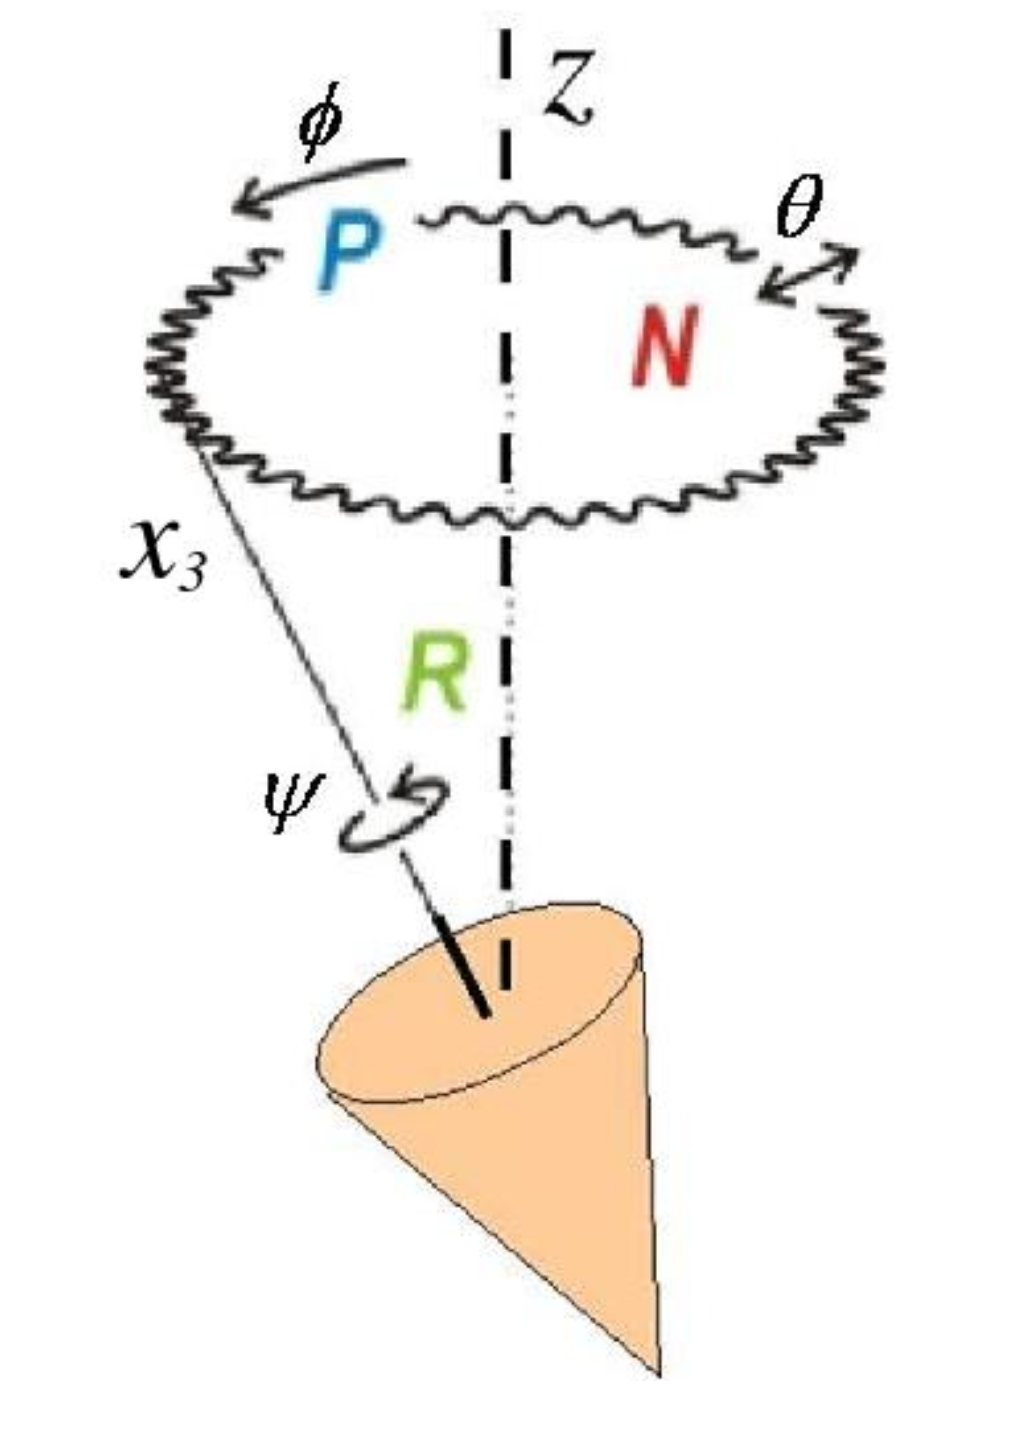
\includegraphics[width=0.9in]{Figuras/PrecesionNutacion.png}
  \end{center}
  \begin{enumerate}
    \item<2-> \textbf{(Nivel 1)} Escriba $\Omega_1,\Omega_2,\Omega_3$ y
          $\Omega_x,\Omega_y,\Omega_z$.
    \item<3-> \textbf{(Nivel 2)} Muestre que $|\bOmega|$, $\bOmega\cdot\uv{x}_3$ y
          $\bOmega\cdot\uv{z}$ son constantes y que $\bOmega$, $\uv{z}$ y $\uv{x}_3$ son
          coplanares. Describa el cono que barre $\bOmega$ en $\Scue$ y en $\Slab$:
          eje, semiángulo y frecuencia de giro con su signo.
    \item<4-> \textbf{(Crítica del enunciado)} Una versión anterior decía: ``gira con
          $\dot\psi_0$ alrededor de $x_3$ formando un ángulo $\theta_0$ con la
          vertical''. ¿Por qué esta frase es ambigua? ¿Qué movimiento resulta si
          inicialmente $\bOmega\parallel\uv{x}_3$?
    \item<5-> \textbf{(Avance)} Con $\vect{L}=\Inercia\,\bOmega$, obtenga $\dot\phi$ y
          $\dot\psi$ en términos de $L$, $I_1$, $I_3$ y $\theta_0$.
  \end{enumerate}
\end{frame}

\begin{frame}
  \frametitle{Para la discusión 2/4: singularidad y rodadura}
  \begin{enumerate}
    \setcounter{enumi}{4}
    \item<1-> \textbf{Singularidad (Nivel 2).} Escriba
          $\colCue{\Omega}=\mathbb{M}(\phi,\theta,\psi)\,(\dot\phi,\dot\theta,\dot\psi)^{\tr}$
          y calcule $\det\mathbb{M}$. Invierta la relación para obtener
          $\dot\phi,\dot\theta,\dot\psi$ en función de $\Omega_1,\Omega_2,\Omega_3$.
          ¿Qué ocurre cuando $\theta\to0$ con $\bOmega$ finito?
    \item<2-> \textbf{Moneda que rueda (Nivel 3).} Un disco delgado de radio $a$
          rueda sin deslizar sobre el plano $z=0$. Su eje de simetría es $x_3$.
      \begin{itemize}
        \item Muestre que $\uv{N}$ está en el plano del disco y que
              $\uv{u}=\uv{x}_3\times\uv{N}$ es el vector unitario del plano del disco
              que apunta hacia arriba.
        \item Escriba la condición de rodadura para el punto de contacto
              $\vect{R}_{\mathrm{cm}}-a\,\uv{u}$ y obtenga $\vect{v}_{\mathrm{cm}}$ en
              términos de $(\phi,\theta,\psi)$ y sus derivadas.
        \item Identifique qué parte de la ligadura es holónoma y qué parte no lo es.
              Justifique.
      \end{itemize}
  \end{enumerate}
\end{frame}

\begin{frame}
  \frametitle{Para la discusión 3/4: auditoría IA (actividad A)}
  \textbf{Actividad con IA requerida (crítica).} A la pregunta ``dame la velocidad
  angular de un cuerpo rígido en ángulos de Euler y su módulo'', un asistente
  respondió (respuesta registrada en clase):
  \begin{exampleblock}{Respuesta del asistente}
    \footnotesize
    ``Con la convención $z$–$x$–$z$, la matriz de rotación es
    $\Rot=\Rot_\phi\Rot_\theta\Rot_\psi$. Las componentes en el cuerpo son
    $\Omega_1=\dot\phi\sen\theta\sen\psi+\dot\theta\cos\psi$,
    $\Omega_2=\dot\phi\sen\theta\cos\psi+\dot\theta\sen\psi$,
    $\Omega_3=\dot\psi+\dot\phi\cos\theta$.
    Como $\bOmega=d\bm{\Phi}/dt$ y $\bm{\Phi}=(\phi,\theta,\psi)$, el módulo es
    $|\bOmega|^2=\dot\phi^2+\dot\theta^2+\dot\psi^2$.''
  \end{exampleblock}
  \begin{itemize}
    \item<2-> \textbf{Discernimiento:} encuentre todos los errores. Para cada uno, nombre
          la verificación que lo detecta: ortogonalidad, límite, invariante, simetría o
          concepto.
    \item<3-> \textbf{Diligencia:} corrija la respuesta. Luego pregunte lo mismo a un
          asistente real, con un prompt \emph{vago} y con uno \emph{preciso}
          (convención, rotación pasiva, sistema de las componentes). Compare.
  \end{itemize}
\end{frame}

\begin{frame}
  \frametitle{Para la discusión 4/4: delegar el cálculo, no la física}
  \textbf{Problema 7 (Nivel 4, IA asistida).} Un cuerpo tiene $\colCue{\Omega}=(\Omega_1,\Omega_2,\Omega_3)$
  constante. Integre la orientación por dos vías: (a) las ecuaciones para
  $(\dot\phi,\dot\theta,\dot\psi)$ del problema 5; (b) la ecuación matricial
  $\dot\Rot=-\tilde{\mathbb{W}}\Rot$. Compare ambas con la solución exacta
  $\Rot(t)=e^{-\tilde{\mathbb{W}}t}\Rot(0)$ cuando el mínimo de $\theta(t)$ se
  acerca a cero.
  \begin{itemize}
    \item<2-> \textbf{Delegación:} usted conserva la convención, el orden del producto,
          la derivación de $\dot\Rot=-\tilde{\mathbb{W}}\Rot$ y la interpretación.
          Delega el código, el álgebra simbólica y los gráficos.
    \item<3-> \textbf{Descripción:} el prompt debe fijar la convención $z$–$x$–$z$ pasiva,
          $\colCue{r}=\Rot\colLab{r}$, el integrador, las tolerancias y las
          condiciones iniciales.
    \item<4-> \textbf{Discernimiento:} verifique $\|\Rot^{\tr}\Rot-\Id\|$, $\det\Rot=+1$,
          $|\bOmega|$ constante, la convergencia al reducir $\Delta t$ y la
          concordancia con la solución exacta.
    \item<5-> \textbf{Diligencia:} entregue la bitácora 4D (prompts; qué aceptó,
          rechazó o corrigió; cómo verificó; errores detectados; razonamiento final),
          el código reproducible y la declaración de uso de IA.
  \end{itemize}
\end{frame}

\begin{frame}
  \frametitle{Política de uso de IA para estas actividades}
  \begin{itemize}
    \item<1-> \textbf{Sin IA:} problemas 1 a 5 (derivación a mano). En clase se
          verifica con una pregunta oral personalizada; por ejemplo, rehacer el
          problema 1 en la convención $z$–$y$–$z$.
    \item<2-> \textbf{IA asistida:} problema 6, solo para el álgebra del producto
          vectorial; el planteamiento de la ligadura es suyo. Problema 7, para el
          código y el álgebra simbólica.
    \item<3-> \textbf{IA requerida:} actividad A, auditoría de la respuesta IA.
    \item<4-> En toda actividad con IA se entrega la bitácora 4D y se evalúa:
          derivación, justificación, verificación, interpretación, reproducibilidad y
          reflexión sobre la interacción.
    \item<5-> Un texto bien escrito no demuestra comprensión. La defensa oral del
          código (explicar una línea elegida por el profesor, cambiar un parámetro en
          vivo) forma parte de la nota.
  \end{itemize}
\end{frame}

% =====================================================================
%  APÉNDICE PARA EL INSTRUCTOR (se incluye solo con \instructortrue)
% =====================================================================
\ifinstructor
\appendix
\section*{Apéndice del instructor}

\begin{frame}
  \frametitle{Instructor: respuestas a las verificaciones conceptuales}
  \footnotesize
  \begin{enumerate}
    \item No. $(\dot\phi,\dot\theta,\dot\psi)$ son componentes sobre la base no ortogonal
          $\{\uv{z},\uv{N},\uv{x}_3\}$, que además depende del tiempo. $\dPhi$ no es una
          diferencial exacta: las rotaciones finitas no conmutan.
    \item $\uv{z}$ tiene proyección $\cos\theta$ sobre $\uv{x}_3$. En cambio,
          $\uv{N}\perp\uv{z}$ siempre, así que $\dot\theta$ nunca contribuye a $\Omega_z$.
    \item Sí. Como $\bOmega\times\bOmega=0$,
          $d\bOmega/dt|_{\Slab}=d\bOmega/dt|_{\Scue}$. Si $\colCue{\Omega}$ es constante,
          $\bOmega$ es un vector fijo también en $\Slab$: el cuerpo gira uniformemente
          alrededor de un eje fijo.
    \item El límite $\Rot(\phi,0,0)=\Rot_\phi$ no lo detecta: vale con cualquier orden.
          Lo detecta la lectura de la tercera fila ($\uv{x}_3$ en $\Slab$): con el orden
          incorrecto depende de $\psi$ y no de $\phi$.
    \item No. Son \emph{cuasi-velocidades}: no existe una terna $(q_1,q_2,q_3)$ con
          $\dot q_i=\Omega_i$, porque $\Omega_i\,dt$ no es una diferencial exacta. El
          lagrangiano se escribe con $(\phi,\theta,\psi)$ como coordenadas
          generalizadas, sustituyendo $\Omega_i(\phi,\theta,\psi,\dot\phi,\dot\theta,\dot\psi)$.
  \end{enumerate}
\end{frame}

\begin{frame}
  \frametitle{Instructor: solución de los problemas 1 a 4 (rotor libre)}
  \footnotesize
  \textbf{Objetivo:} 3 (componentes de $\bOmega$). \textbf{Conceptos:} proyecciones,
  conos de Poinsot, elección de ejes. \textbf{Dificultad:} 1–2; el ítem 4 es avance.
  \begin{enumerate}
    \item Con $\theta=\theta_0$ y $\dot\theta=0$:
      $\Omega_1=\dot\phi\sen\theta_0\sen\psi$, $\Omega_2=\dot\phi\sen\theta_0\cos\psi$,
      $\Omega_3=\dot\psi+\dot\phi\cos\theta_0$;\;
      $\Omega_x=\dot\psi\sen\theta_0\sen\phi$, $\Omega_y=-\dot\psi\sen\theta_0\cos\phi$,
      $\Omega_z=\dot\phi+\dot\psi\cos\theta_0$.
    \item $\bOmega=\dot\phi\,\uv{z}+\dot\psi\,\uv{x}_3$ es coplanar con $\uv{z}$ y
      $\uv{x}_3$. $|\bOmega|^2=\dot\phi^2+\dot\psi^2+2\dot\phi\dot\psi\cos\theta_0$
      es constante, y también lo son $\Omega_3$ y $\Omega_z$.
      \textbf{Cono del cuerpo:} eje $x_3$; $(\Omega_1,\Omega_2)=\dot\phi\sen\theta_0(\sen\psi,\cos\psi)$
      gira con velocidad angular $-\dot\psi\,\uv{x}_3$; semiángulo
      $\arctan(|\dot\phi|\sen\theta_0/|\Omega_3|)$.
      \textbf{Cono espacial:} eje $z$; $(\Omega_x,\Omega_y)=\dot\psi\sen\theta_0(\sen\phi,-\cos\phi)$
      gira con $+\dot\phi\,\uv{z}$; semiángulo $\arctan(|\dot\psi|\sen\theta_0/|\Omega_z|)$.
    \item Si al inicio $\bOmega=\dot\psi_0\uv{x}_3$, entonces $\vect{L}=I_3\dot\psi_0\uv{x}_3$
      y la rotación es estacionaria alrededor de $x_3$: no hay precesión. Además,
      ``vertical'' carece de significado sin campo externo. Para que $\theta_0$ sea
      constante con precesión no nula, hay que tomar $z\parallel\vect{L}$ y
      $\bOmega\not\parallel\uv{x}_3$.
    \item $L_i=I_i\Omega_i$ y $\uv{z}$ en $\Scue$:
      $I_1\dot\phi\sen\theta_0\sen\psi=L\sen\theta_0\sen\psi\Rightarrow\dot\phi=L/I_1$;\;
      $I_3(\dot\psi+\dot\phi\cos\theta_0)=L\cos\theta_0\Rightarrow
      \dot\psi=L\cos\theta_0\,(I_1-I_3)/(I_1I_3)$.
  \end{enumerate}
  \textbf{Errores frecuentes:} tomar $z$ arbitrario; suponer
  $|\bOmega|^2=\dot\phi^2+\dot\psi^2$; equivocar el signo del giro del cono del cuerpo.
  \textbf{Pista:} use $\bOmega=\dot\phi\uv{z}+\dot\psi\uv{x}_3$.
  \textbf{Extensión:} prolato ($I_3<I_1$) frente a oblato; signo de $\dot\psi$.
\end{frame}

\begin{frame}
  \frametitle{Instructor: solución del problema 5 (singularidad)}
  \footnotesize
  \textbf{Problema 5} (objetivo 4; nivel 2).
  \[
    \mathbb{M}=\begin{pmatrix}\sen\theta\sen\psi&\cos\psi&0\\ \sen\theta\cos\psi&-\sen\psi&0\\ \cos\theta&0&1\end{pmatrix},
    \qquad \det\mathbb{M}=-\sen\theta .
  \]
  Inversa:
  \[
    \dot\phi=\frac{\Omega_1\sen\psi+\Omega_2\cos\psi}{\sen\theta},\qquad
    \dot\theta=\Omega_1\cos\psi-\Omega_2\sen\psi,
  \]
  \[
    \dot\psi=\Omega_3-\cot\theta\,(\Omega_1\sen\psi+\Omega_2\cos\psi).
  \]
  Si $\theta\to0$ con $\bOmega$ finito, $\dot\phi$ y $\dot\psi$ divergen con signos
  opuestos y $\dot\phi+\dot\psi$ permanece finito. La divergencia es de la carta de
  coordenadas, no física.
  \textbf{Error frecuente:} concluir que el cuerpo ``gira infinitamente rápido''.
  \textbf{Pista:} mire primero el bloque $2\times2$ superior izquierdo de $\mathbb{M}$.
  \textbf{Extensión:} repita con la convención $x$–$y$–$z$ y localice su singularidad.
\end{frame}

\begin{frame}
  \frametitle{Instructor: solución del problema 6 (moneda que rueda)}
  \footnotesize
  \textbf{Problema 6} (objetivos 1 y 3; nivel 3; conceptos: ligaduras, $\bOmega\times\vect{r}$).
  \textbf{Estrategia:} geometría del contacto, luego condición de rodadura y proyección.

  \medskip $\uv{N}\perp\uv{x}_3$, así que
  $\uv{N}$ está en el plano del disco; además es horizontal. Con
  $\uv{u}=\uv{x}_3\times\uv{N}=(-\cos\theta\sen\phi,\cos\theta\cos\phi,\sen\theta)$,
  $u_z=\sen\theta\ge0$. Rodadura: $\vect{v}_{\mathrm{cm}}+\bOmega\times(-a\uv{u})=0$,
  es decir, $\vect{v}_{\mathrm{cm}}=a\,\bOmega\times\uv{u}$. Proyectando:
  \[
    \vect{v}_{\mathrm{cm}}\cdot\uv{N}=-a\,\Omega_3=-a(\dot\psi+\dot\phi\cos\theta),\quad
    \vect{v}_{\mathrm{cm}}\cdot(\uv{z}\times\uv{N})=-a\sen\theta\,\dot\theta,\quad
    \dot Z=a\cos\theta\,\dot\theta .
  \]
  La ecuación para $\dot Z$ se integra: $Z=a\sen\theta$ (holónoma). Las horizontales,
  $\dot X\cos\phi+\dot Y\sen\phi=-a(\dot\psi+\dot\phi\cos\theta)$ y su compañera, no
  son integrables (no holónomas): a una misma configuración final se puede llegar
  por caminos de rodadura distintos. \textbf{Verificación:} si $\theta=\pi/2$ y $\dot\theta=0$, entonces
  $|\vect{v}_{\mathrm{cm}}|=a|\dot\psi|$ a lo largo de $\uv{N}$.
  \textbf{Errores frecuentes:} usar $+a\uv{u}$ para el contacto; omitir $\dot\phi\cos\theta$.
  \textbf{Extensión:} moneda que rueda en círculo con $\theta$ constante.
\end{frame}

\begin{frame}
  \frametitle{Instructor: clave de la actividad A (auditoría IA)}
  \footnotesize
  \begin{enumerate}
    \item \textbf{Orden del producto:} $\Rot_\phi\Rot_\theta\Rot_\psi$ es incorrecto en la
          convención pasiva $\colCue{r}=\Rot\colLab{r}$. Se detecta porque la tercera
          fila (que debe ser $\uv{x}_3$ en $\Slab$) depende de $\psi$ y no de $\phi$.
    \item \textbf{Signo en $\Omega_2$:} debe ser $-\dot\theta\sen\psi$. Se detecta con
          $|\bOmega|^2$: con el signo erróneo aparece el término cruzado
          $4\dot\theta\dot\phi\sen\theta\sen\psi\cos\psi$, que depende de $\psi$.
          Pero $\Omega_x,\Omega_y,\Omega_z$ no dependen de $\psi$, así que el módulo
          tampoco puede depender de $\psi$. También se detecta con $\uv{N}=(\cos\psi,-\sen\psi,0)$ en $\Scue$.
    \item \textbf{Concepto:} $\bm{\Phi}=(\phi,\theta,\psi)$ no es un vector (no
          conmutatividad). Error derivado: el módulo omite $2\dot\phi\dot\psi\cos\theta$.
          Se detecta con el límite $\theta=0$, $\dot\theta=0$, donde debe valer $|\bOmega|=|\dot\phi+\dot\psi|$.
    \item Lo correcto (debe aceptarse): $\Omega_1$ y $\Omega_3$.
  \end{enumerate}
  \textbf{Error frecuente del estudiante:} corregir solo la fórmula del módulo sin
  identificar el error conceptual que la produce.
\end{frame}

\begin{frame}
  \frametitle{Instructor: rúbrica de la actividad A}
  \footnotesize
  Cada criterio se califica de 0 a 3:

  \medskip
  \begin{tabular}{p{2.2cm}p{8.6cm}}
    Detección & 3: identifica los 3 errores y acepta lo correcto con razones;
                2: identifica 2; 1: identifica 1; 0: ninguno o acepta todo. \\
    Verificación & 3: cada error con una prueba independiente nombrada y ejecutada;
                   2: pruebas correctas pero sin ejecutar; 1: argumento de autoridad;
                   0: ninguna. \\
    Corrección & 3: respuesta corregida y rederivada a mano; 2: corregida sin
                 derivación; 1: parcial; 0: ninguna. \\
    Bitácora 4D & 3: prompts vago y preciso, comparación y reflexión sobre la
                  convención; 2: falta la comparación; 1: solo prompts; 0: ausente. \\
    Defensa oral & 3: explica sin apoyo por qué cada verificación detecta su error;
                   2: con apoyo; 1: solo repite el texto entregado; 0: no puede explicar.
  \end{tabular}
\end{frame}

\begin{frame}[fragile]
  \frametitle{Instructor: implementación de referencia del problema 7}
\begin{lstlisting}
import numpy as np
from scipy.integrate import solve_ivp
from scipy.linalg import expm

def A_euler(phi, th, psi):                 # A = A_psi A_theta A_phi  (S -> S~, pasiva)
    c, s = np.cos, np.sin
    Rz = lambda a: np.array([[c(a), s(a), 0], [-s(a), c(a), 0], [0, 0, 1]])
    Rx = lambda a: np.array([[1, 0, 0], [0, c(a), s(a)], [0, -s(a), c(a)]])
    return Rz(psi) @ Rx(th) @ Rz(phi)

def hat(w):                                # hat(w) @ v = w x v
    return np.array([[0, -w[2], w[1]], [w[2], 0, -w[0]], [-w[1], w[0], 0]])

Om = np.array([1.0, 0.0, 0.05])            # componentes en el cuerpo [1/s]
q0 = np.array([0.0, 0.4, 0.0])             # (phi, theta, psi) iniciales [rad]

def rhs_euler(t, q):                       # inversa del problema 5
    phi, th, psi = q
    S = (Om[0]*np.sin(psi) + Om[1]*np.cos(psi)) / np.sin(th)
    return [S, Om[0]*np.cos(psi) - Om[1]*np.sin(psi), Om[2] - np.cos(th)*S]

def rhs_matrix(t, y):                      # dA/dt = -hat(Om) A
    return (-hat(Om) @ y.reshape(3, 3)).ravel()

T, tol = 20.0, dict(method="DOP853", rtol=1e-10, atol=1e-12)
te = np.linspace(0, T, 2001)
se = solve_ivp(rhs_euler,  (0, T), q0, t_eval=te, **tol)
sm = solve_ivp(rhs_matrix, (0, T), A_euler(*q0).ravel(), t_eval=te, **tol)
exact = np.array([expm(-hat(Om)*t) @ A_euler(*q0) for t in te])
Ae, Am = np.array([A_euler(*q) for q in se.y.T]), sm.y.T.reshape(-1, 3, 3)
print("error Euler :", np.abs(Ae - exact).max(), " evaluaciones:", se.nfev)
print("error matriz:", np.abs(Am - exact).max(), " evaluaciones:", sm.nfev)
print("max |A^T A - I|:", max(np.abs(A.T @ A - np.eye(3)).max() for A in Am))
\end{lstlisting}
\end{frame}

\begin{frame}
  \frametitle{Instructor: resultados esperados del problema 7}
  \footnotesize
  Resultados con $\Omega_1=1\,\mathrm{s}^{-1}$, $\Omega_2=0$, $\theta_0=0.4$,
  $T=20\,\mathrm{s}$. La columna DOP853 sale del script anterior; las columnas RK4,
  de un RK4 de paso fijo que escriben los estudiantes. Los valores pueden variar
  ligeramente con la plataforma:
  \begin{center}
  \resizebox{\textwidth}{!}{%
  \begin{tabular}{ccccc}
    & & \multicolumn{2}{c}{error máx. RK4 (Euler / matriz)} & DOP853: evaluaciones \\
    $\Omega_3$ [s$^{-1}$] & $\min\theta$ [rad] & $\Delta t=0.05$ & $\Delta t=0.01$ &
    (Euler / matriz)\\ \hline
    0.30 & $2.4\times10^{-2}$ & $6\times10^{-3}$ / $1\times10^{-6}$ & $7\times10^{-6}$ / $2\times10^{-9}$ & 4949 / 1061\\
    0.05 & $4.0\times10^{-3}$ & $0.46$ / $1\times10^{-6}$ & $1\times10^{-3}$ / $2\times10^{-9}$ & 7193 / 962\\
    0.01 & $1.6\times10^{-3}$ & $0.15$ / $1\times10^{-6}$ & $2\times10^{-2}$ / $2\times10^{-9}$ & 9284 / 932
  \end{tabular}}
  \end{center}
  \begin{itemize}
    \item \textbf{Interpretación esperada:} cerca de $\theta=0$ el lado derecho crece
          como $1/\sen\theta$: con paso fijo el error crece varios órdenes de magnitud y
          con paso adaptativo se multiplica el costo. La formulación matricial no
          percibe la singularidad: es un \textbf{artefacto de la carta}, no física.
    \item \textbf{Errores frecuentes:} signo en $\dot\Rot=-\tilde{\mathbb{W}}\Rot$;
          comparar ángulos en vez de matrices (saltos de $2\pi$, ambigüedad en
          $\theta\approx0$); no verificar la ortogonalidad.
    \item \textbf{Rúbrica sugerida:} derivación de $\dot\Rot=-\tilde{\mathbb{W}}\Rot$ (25\%),
          verificación y convergencia (25\%), interpretación del artefacto (25\%),
          bitácora 4D y defensa oral del código (25\%).
    \item \textbf{Extensión:} cuaterniones unitarios; ángulos de Tait–Bryan $x$–$y$–$z$.
  \end{itemize}
\end{frame}
\fi

\end{document}
